%\VignetteIndexEntry{contextual: Simulating Contextual Multi-Armed Bandit Problems in R (article)}
%\VignetteEngine{knitr::knitr}
%\VignetteKeyword{archivsit}
%\VignetteKeyword{package}
%\VignetteKeyword{vignette}
%\VignetteKeyword{LaTeX}
\documentclass[nojss]{jss}\usepackage[]{graphicx}\usepackage[]{color}
%% maxwidth is the original width if it is less than linewidth
%% otherwise use linewidth (to make sure the graphics do not exceed the margin)
\makeatletter
\def\maxwidth{ %
  \ifdim\Gin@nat@width>\linewidth
    \linewidth
  \else
    \Gin@nat@width
  \fi
}
\makeatother

\definecolor{fgcolor}{rgb}{0.345, 0.345, 0.345}
\newcommand{\hlnum}[1]{\textcolor[rgb]{0.686,0.059,0.569}{#1}}%
\newcommand{\hlstr}[1]{\textcolor[rgb]{0.192,0.494,0.8}{#1}}%
\newcommand{\hlcom}[1]{\textcolor[rgb]{0.678,0.584,0.686}{\textit{#1}}}%
\newcommand{\hlopt}[1]{\textcolor[rgb]{0,0,0}{#1}}%
\newcommand{\hlstd}[1]{\textcolor[rgb]{0.345,0.345,0.345}{#1}}%
\newcommand{\hlkwa}[1]{\textcolor[rgb]{0.161,0.373,0.58}{\textbf{#1}}}%
\newcommand{\hlkwb}[1]{\textcolor[rgb]{0.69,0.353,0.396}{#1}}%
\newcommand{\hlkwc}[1]{\textcolor[rgb]{0.333,0.667,0.333}{#1}}%
\newcommand{\hlkwd}[1]{\textcolor[rgb]{0.737,0.353,0.396}{\textbf{#1}}}%
\let\hlipl\hlkwb

\usepackage{framed}
\makeatletter
\newenvironment{kframe}{%
 \def\at@end@of@kframe{}%
 \ifinner\ifhmode%
  \def\at@end@of@kframe{\end{minipage}}%
  \begin{minipage}{\columnwidth}%
 \fi\fi%
 \def\FrameCommand##1{\hskip\@totalleftmargin \hskip-\fboxsep
 \colorbox{shadecolor}{##1}\hskip-\fboxsep
     % There is no \\@totalrightmargin, so:
     \hskip-\linewidth \hskip-\@totalleftmargin \hskip\columnwidth}%
 \MakeFramed {\advance\hsize-\width
   \@totalleftmargin\z@ \linewidth\hsize
   \@setminipage}}%
 {\par\unskip\endMakeFramed%
 \at@end@of@kframe}
\makeatother

\definecolor{shadecolor}{rgb}{.97, .97, .97}
\definecolor{messagecolor}{rgb}{0, 0, 0}
\definecolor{warningcolor}{rgb}{1, 0, 1}
\definecolor{errorcolor}{rgb}{1, 0, 0}
\newenvironment{knitrout}{}{} % an empty environment to be redefined in TeX

\usepackage{alltt}

\usepackage[utf8]{inputenc}
\usepackage{color}

%% packages added by RvE
\usepackage{amssymb}
\usepackage{amsmath}
\usepackage{txfonts}
\usepackage{mathdots}
\usepackage{float}
\usepackage{algorithm}
\usepackage{algorithmic}
%\usepackage[classicReIm]{kpfonts}
%\usepackage[pdftex]{graphicx}

\DeclareMathOperator*{\argmax}{arg\,max}

\usepackage{natbib}
\usepackage[british]{babel} % for correct word hyphenation
\raggedbottom % for blank spaces at the bottom (e.g., references section)
%\setcounter{tocdepth}{3} % for table of contents
%\setcounter{secnumdepth}{3} % setting level of numbering
%%%%%%%%%%%%%%%%%%%%%%%%%%%%%%
%% declarations for jss.cls %%%%%%%%%%%%%%%%%%%%%%%%%%%%%%%%%%%%%%%%%%
%%%%%%%%%%%%%%%%%%%%%%%%%%%%%%

%% almost as usual
\author{Robin van Emden\\JADS \And
  Eric Postma\\Tilburg University \And
  Maurits Kaptein\\Tilburg University}

\title{\pkg{contextual}: Simulating Contextual Multi-Armed Bandit Problems in R}

%% for pretty printing and a nice hypersummary also set:
\Plainauthor{Robin van Emden, Eric Postma, Maurits Kaptein} %% comma-separated
\Plaintitle{contextual: Simulating Contextual Multi-Armed Bandit Problems in R} %% without formatting
\Shorttitle{\pkg{contextual}} %% a short title (if necessary)



%% an abstract and keywords
\Abstract{

Contextual bandit algorithms have been gaining in popularity due to their effectiveness and flexibility in the online evaluation of partial information sequential decision problems - from online advertising and recommender systems to clinical trial design and personalized medicine. At the same time, there are as of yet surprisingly few options that enable researchers and practitioners to simulate and compare the wealth of new and existing Bandit algorithms in a practical, standardized and extensible way. To help close this gap between analytical research and real-life application the current paper introduces the object-oriented R package \pkg{contextual}: a user-friendly and, through its clear object oriented structure, easily extensible framework that facilitates the parallel comparison of contextual and non-contextual Bandit policies by means of both simulation and offline analysis.
}

\Keywords{contextual multi-armed bandits, simulation, sequential experimentation, \proglang{R}}
\Plainkeywords{contextual multi-armed bandits, simulation, sequential experimentation, R}

%% at least one keyword must be supplied

%% publication information
%% NOTE: Typically, this can be left commented and will be filled out by the technical editor
%% \Volume{50}
%% \Issue{9}
%% \Month{June}
%% \Year{2012}
%% \Submitdate{2012-06-04}
%% \Acceptdate{2012-06-04}

%% The address of (at least) one author should be given
%% in the following format:
\Address{
  Robin van Emden\\
  Jheronimus Academy of Data Science\\
  Den Bosch, the Netherlands\\
  E-mail: \email{robin@pwy.nl} \\
  URL: \url{pavlov.tech}\\
  \linebreak
  Eric O. Postma\\
  Tilburg University\\
  Communication and Information Sciences\\
  Tilburg, the Netherlands\\
  E-mail: \email{e.o.postma@tilburguniversity.edu}\\
  \linebreak
  Maurits C. Kaptein\\
  Tilburg University\\
  Statistics and Research Methods\\
  Tilburg, the Netherlands\\
  E-mail: \email{m.c.kaptein@uvt.nl}\\
  URL: \url{www.mauritskaptein.com}\\
}

%% It is also possible to add a telephone and fax number
%% before the e-mail in the following format:
%% Telephone: +43/512/507-7103
%% Fax: +43/512/507-2851

%% for those who use Sweave please include the following line (with % symbols):
%% need no \usepackage{Sweave.sty}

%% end of declarations %%%%%%%%%%%%%%%%%%%%%%%%%%%%%%%%%%%%%%%%%%%%%%%
\IfFileExists{upquote.sty}{\usepackage{upquote}}{}
\begin{document}

%% A vignette for the \cite{contextual} paper. #########################################

%% include your article here, just as usual
%% Note that you should use the \pkg{}, \proglang{} and \code{} commands.





\section{Introduction}
%% Note: If there is markup in \(sub)section, then it has to be escape as above.

There are many real-world situations in which we have to decide between a set of options but only learn about the best course of action by choosing one way or the other repeatedly, learning but one step at a time. In such situations, the basic premise stays the same for each renewed decision: do you stick to what you already know and receive an expected result ("exploit") or choose something you don't know all that much about and potentially learn something new ("explore")? As we all encounter such dilemma's on a daily basis, it is easy to come up with many examples - for instance:

\begin{itemize}
\item Do you feed your next coin to the one-armed bandit that paid out last time, or do you test your luck on another arm, on another machine?
\item When going out to dinner, do you explore new restaurants, or do you exploit familiar ones?
\item Do you stick to your current job, or explore and hunt around?
\item Do I keep my current stocks, or change my portfolio and pick some new ones?
\item As an online marketer, do you try a new ad, or keep the current one?
\item As a doctor, do you treat your patients with tried and tested medication, or do you prescribe a new and promising experimental treatment?
\end{itemize}

Every one of these issues represents another take on the same underlying dilemma: when to explore, versus when to exploit. To get a better grip on such decision problems, and to learn if and when specific strategies might be more successful than others, such explore/exploit dilemmas have been studied extensively under the umbrella of the "Multi-Armed Bandit" problem (MAB problem). Here, an algorithm or "policy" repeatedly selects one out of a limited set of options or "arms," each with its particular (hidden) payout distribution. Every time the policy selects another arm, it will receive a reward from the "multi-armed bandit," which represents all available arms together with their hidden reward distributions. The policy itself continuously seeks to maximize its average rewards over time by balancing the exploration of arms with more uncertain payoffs with the exploitation of arms that offer the highest current expected payoff. Importantly, on each repeated choice, the policy only reveives a reward for the chosen arm: he or she remains in the dark about the potential rewards of the unchosen arms.

A recent MAB generalization known as the \textit{contextual} Multi-Armed Bandit (cMAB) builds on this formalization by adding one crucial element: contextual information. That is, cMAB policies make use of side information on the state of the world at each repeated time step t. This access to side information makes cMAB algorithms even more relevant to many real-life decision problems than its MAB progenitors: do you show a particular add to returning customers, to new ones, or both? Do you prescribe a different treatment to male patients, female patients, or both? In the real world, it appears almost no choice exists without a context. So it may be no surprise that cMAB algorithms have found many applications: from recommender systems and advertising to health apps and personalized medicine - inspiring a multitude of new, often analytically derived bandit algorithms or policies, each with their strengths and weaknesses.

Still, though cMAB algorithms have gained traction in both research and industry, comparisons on simulated, and, importantly, real-life, large-scale offline \textquotedblleft{}partial label\textquotedblright{} data sets have relatively lagged behind. To this end, the current paper introduces the \pkg{contextual} R package. \pkg{contextual} aims to facilitate the simulation, offline comparison, and evaluation of (Contextual) Multi-Armed bandit policies. There exist a few other frameworks that enable the analysis of offline datasets in some capacity, such as Microsoft's Vowpal Wabbit, and the MAB focussed python package Striatum. But, as of yet, no extensible and widely applicable R package that can analyze and compare, respectively, K-armed, Continuum, Adversarial and Contextual Multi-Armed Bandit Algorithms on either simulated or offline data.

In section 2, this paper will continue with a more formal definition of MAB and CMAB problems and relate it to our implementation. In section 3, we will continue with an overview of \pkg{contextual}’s object-oriented structure In section 4, we list the policies that are available by default, and simulate two MAB policies and a cMAB policy. In section 5, we demonstrate how easy it is to extend \pkg{contextual} with a policy (RVE: NOTE TO SELF: also custom bandit?) of your own. In section 6, we replicate two papers, thereby demonstrating how to test policies on offline data sets. Finally, in section  7, we will go over some of the additional features in the package and conclude with some comments on the current state of the package and possible enhancements.


\section{From formalisation to implementation}
%% Note: If there is markup in \(sub)section, then it has to be escape as above.


\subsection{Formalisation}


In formalizing the described cMAB problem, a (k-armed) \textbf{bandit} $\mathfrak{B}$ can be defined as a set of $k$ distributions $\mathfrak{B}=\{D_{1},\dots ,D_{k}\}$, where each distribution is associated with the I.I.D. rewards generated by one of the $k\in \mathbb {N} ^{+}$ arms. We now define an algorithm or \textbf{policy} $\piup$, that seeks to maximize its total \textbf{reward} (that is, to maximize its cumulative reward $\sum_{t=1}^T r_t$ or minimize its cumulative regret---see equation \ref{eq:1}). This \textbf{policy} observes information on the current state of the world represented as a $d$-dimensional contextual feature vector \(x_{t}=\left( x_{1,t},  \dots, x_{d,t}\right)\). Based on earlier payoffs, the \textbf{policy} then selects one of the \textbf{bandit} $\mathfrak{B}$'s arms by choosing an action a \(a_{t} \in \left\{ 1, \dots, k \right\}\), and receives reward \(r_{a_{t},t}\), the expectation of which depends both the context and the reward history of that particular arm. With this observation \( (x_{t,a_t},a_{t},r_{t,a_t}) \), the policy now updates its arm-selection strategy through some investigation of how these contexts, actions and rewards hang together. These steps are then repeated \textit{T} times, where \textit{T} is often named the \textbf{horizon}.

Schematically, for each round \emph{t}= \{1, \ldots, T\}:

\begin{enumerate}
         \item[1)] Policy $\piup$ observes state of the world as contextual feature vector \(x_{t}=\left( x_{1,t},  \dots, x_{d,t}\right)\)
         \item[2)] Bandit $\mathfrak{B}$ generates reward vector \(r_{t}=\left( r_{t,1},  \dots, r_{t,k}\right)\)
         \item[3)] Policy $\piup$ selects one of bandit $\mathfrak{B}$'s arms \(a_{t} \in \left\{ 1, \dots, k \right\}\)
         \item[4)] Policy $\piup$ observes reward \(r_{t,a_t}\) from bandit $\mathfrak{B}$ and updates its arm-selection strategy with \( (x_{t,a_t},a_{t},r_{t,a_t}) \)
\end{enumerate}

Where the goal of the policy $\piup$ is to miminize its cumulative regret over \emph{t}= \{ 1, \ldots, T \}, defined as the sum of rewards that would have been received by always choosing optimal actions $a^{*}$ over \emph{t} subtracted by the sum of rewards awarded to the actually chosen actions $a$ over \emph{t}:

\begin{equation} \label{eq:1}
R^{\pi}_{T} = \max_{a^{*}= 1, \dots, k} \sum^{T}_{t=1}(r_{a^{*}_t,x_t}) - \sum^{T}_{t=1}(r^{\pi}_{a_t,x_t})
\end{equation}

\subsection{Basic Implementation}

We set out to develop an implementation that stays close to the previous formalisation, while offering maximum flexibility and extendibility. As an added bonus, this kept the class structure of the package elegant and simple, with the following five classes forming the backbone of the package:

\begin{itemize}
         \item \code{Bandit}: generates rewards and contexts. These can be generated synthetically, based on offline data, etc.
         \item \code{Policy}: observes the context and the rewards of a \code{Bandit}, uses these observations to update of a set of parameters $\theta$, and decides which arm to choose next.
         \item \code{Agent}: takes care of the flow of information between and the running of one \code{Bandit}/\code{Policy} pair.
         \item \code{Simulation}: the entry point of any \pkg{contextual} simulation. It encapsulates one or more \code{Agents}, clones them if necessary, runs the \code{Agents}, and saves the log of all of the \code{Agents} interactions to a \code{History} object.
         \item \code{History}: encapsulates an R \code{data.table}, keeps a log of all interactions, and provides data summaries.
         \item \code{Plot}: generates plots based on \code{History} data. It can also be invoked by calling the generic \code{plot(h)}, where \code{h} is an \code{History} class instance.
\end{itemize}

Importantly, any particular \code{Bandit} or \code{Policy} class has to inherit from, and implement the functions of, its respective abstract superclass. From this follows that in our framework, on being run by the Simulator, an Agent repeatedly performs the following operations at every \textit{t} in \textit{t}=1,2,{\dots},\textit{T} (see also Figure ~\ref{fig:cmab_chart})

\begin{enumerate}
         \item[1a)] \code{Agent} asks the \code{Bandit} for side information that might influence the expression of its arms.
         \item[1b)] \code{Bandit} returns feature vector \textit{Xt}.
         \item[2a)] \code{Agent} asks \code{Policy} $\piup$ which of the \code{Bandit}'s k arms to choose given \textit{Xt}.
         \item[2b)] Given \textit{Xt}, \code{Policy} $\piup$ advices action \textit{a${}_{t}$} based on the state of a set of parameters \textit{$\theta$${}_{t}$${}_{  }$}.
         \item[3a)] \code{Agent} does action \textit{a${}_{t}$} by playing the suggested \code{Bandit} arm.
         \item[3b)] \code{Bandit} rewards the \code{Agent} with reward \textit{r${}_{t}$ }for action \textit{a${}_{t}$}.
         \item[4a)] The \code{Agent} sends the reward\textit{ r${}_{t}$ }to \code{Policy} $\piup$.
         \item[4b)] \code{Policy} $\piup$ uses \textit{r${}_{t}$} to update the \code{Policy}'s set of parameters\textit{ $\theta$${}_{t}$${}_{  }$} given \textit{Xt}.
\end{enumerate}

Where we assume that at each time step t, all information necessary to choose an arm is summarized using a limited set of parameters denoted $\theta_t$, whose dimensionality is much smaller than of the log of all historical interactions.

\begin{figure}[H]
  \centering
    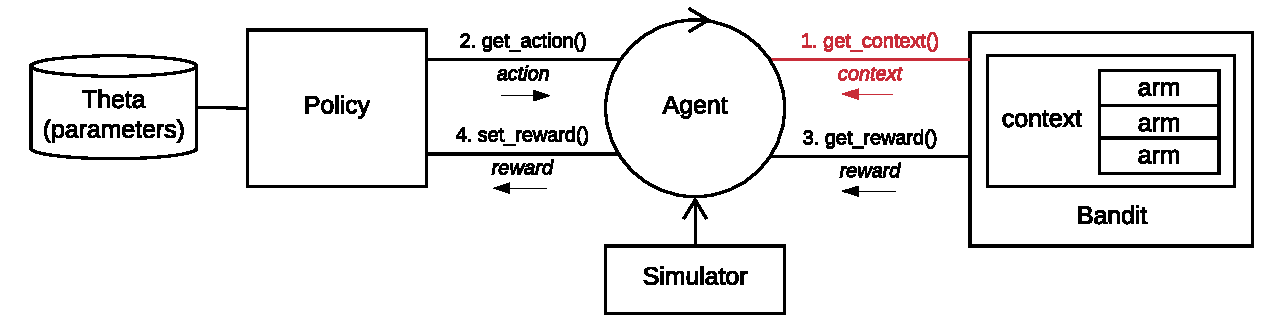
\includegraphics[width=.99\textwidth]{fig/cmab_chart}
    \label{fig:cmab_chart}
      \caption{Basic model of the logical flow of an \pkg{contextual}. The extension from MAB towards cMAB models is higlighted in red. }
\end{figure}











\section{Object-oriented setup of the package}
%% Note: If there is markup in \(sub)section, then it has to be escape as above.

\subsection{R6 Class System}


Statistical computational methods, in R or otherwise,  are regularly made available through single-use scripts or basic, isolated code packages. Usually, such code examples are meant to give a basic idea of a statistical method, technique or algorithm in the context of a scientific paper.  Such code examples offer their scientific audience a rough inroad towards the comparison and further implementation of their underlying methods. But when a set of well-researched interrelated algorithms, such as MAB and cMAB policies, find growing academic, practical and commercial adoption, it becomes crucial to offer a more standardized and more accessible way to compare such methods and algorithms.

It is against this background that we decided to develop the \pkg{contextual} R package--a package that offers an easily extendible and open bandit framework together with an extensible bandit library that presents some of the most well known and popular bandit algorithms. To us, it made the most sense to create such a package in R, as R is currently the de facto language for the dissemination of new statistical methods, techniques, and algorithms--while it is at the same time finding ever-growing adoption in industry. The resulting lively exchange of R related code, data, and knowledge between scientists in both academia and business offers precisely the kind of cross-pollination that \pkg{contextual} hopes to facilitate.

Given this background, it was of critical importance to make our R based framework as concise and as easily extensible as possible. For us, this meant it made the most sense to build our package on the relatively new R6 object system, as the R6 system allowed us to create readily intelligible, coherent classes that made use of R6's reference semantics. These reference semantics are similar to R's built-in reference classes. But compared to these classes, the resulting R6 classes are simpler and lighter-weight, and (as they are not built on S4 classes) do not require the methods package. This made \pkg{contextual} substantially less resource-hungry and its resulting objects much smaller than they would otherwise have been--of great importance in a simulation package such as \pkg{contextual}.

Another, more general advantage of making use of an object system such as the R6 system is that such systems support class inheritance. In other words, we were able to create subclasses (for example, ContextualBandit) that can add or override methods to their superclasses (for example, Bandit). This enabled us to translate the cMAB formalization from section 2 almost one on one to a transparent object-oriented structure.

To clarify the resulting class structure, we have created two UML diagrams (UML, or "Unified Modeling Language" is a modeling language that presents a standard way to visualize the overall class structure and general design of a software application or framework). The UML class diagram shown in figure X visualizes the structure of our package by showcasing the most important of \pkg{contextual}'s classes, attributes, and relationships at rest. The UML sequence diagram in figure X, on the other hand, shows how \pkg{contextual}'s classes behave over time. This diagram depicts a basic overview of the sequence of function calls between some of \pkg{contextual}'s main objects in action.


\subsection{Main classes}

At least policy, and often the bandit, ...Two of the classes more in depth, as those are the ones that generally need to be extended for the evaluation of Policies. Let's now take a closer look at both UML diagrams, and go over each of our classes one by one.

\subsubsection{Bandit}

The abstract class \code{Bandit} is the super class of any \code{Bandit} subclass that is to be implemented in \pkg{contextual}. As it is an abstract class, it declares methods, but contains no implementation. That is, every \code{Bandit} class in the \pkg{contextual} package inherits from and has to implement the methods of by this class.

In practice, this implies that any \code{Bandit} subclass needs to set \code{self\$k} to the number of arms, and \code{self\$d} to the number of context features during its initialisation. On meeting this requirement, the \code{Bandit} is then required to implement \code{get_context()} and \code{do_action()}:

\begin{knitrout}\small
\definecolor{shadecolor}{rgb}{0.969, 0.969, 0.969}\color{fgcolor}\begin{kframe}
\begin{alltt}
Bandit <- R6::\hlkwd{R6Class}(
  public = \hlkwd{list}(
    k             = NULL,  \hlcom{# number of \hlkwd{arms} (integer)}
    d             = NULL,  \hlcom{# dimension of context \hlkwd{feature} (integer)}
    precaching    = FALSE, \hlcom{# pregenerate context & reward matrices? (boolean)}

    get_context = \hlkwd{function}(t) \{
      \hlkwd{stop}(\hlstr{"Bandit subclass needs to implement bandit$\hlkwd{get_context}()"})
\hlcom{      # return a list with self$k, self$d and, where applicable, context vector X.}
      \hlkwd{list}(k = n_arms, d = n_features, X = context)
    \},
    do_action = \hlkwd{function}(action, t) \{
      \hlkwd{stop}(\hlstr{"Bandit subclass needs to implement bandit$\hlkwd{do_action}()"})
\hlcom{      # return a list with the reward and, if known, the reward of the best arm.}
      \hlkwd{list}(reward = reward_for_choice_made, optimal = optimal_reward)
    \},
    generate_bandit_data = \hlkwd{function}(n) \{
\hlcom{      # called when precaching is TRUE. Pregenerates contexts and rewards.}
      \hlkwd{stop}("Bandit subclass needs to implement bandit$\hlkwd{generate_cache}()
           when bandit$precaching is TRUE.",
    \}
  )
)
\end{alltt}
\end{kframe}
\end{knitrout}

Where possible, it is advisable to pregenerate or precache Bandit contexts and rewards, as this is computationally much more efficient than the repeated generation of these vectors. To facilitate this, during initialisation \pkg{contextual} calls \code{generate_bandit_data()} for every Bandit where \code{self$precaching} is \code{TRUE}.

\pkg{contextual} makes several Bandits available out of the box. For each Bandit, there is at least one example script, to be found in the package's  \code{demo} directory. The currently available Bandits are:

\begin{itemize}
         \item \code{BasicBandit}: this basic k-armed bandit synthetically generates rewards based on a weigh vector that has to set at instantiation. It does not return context vector X.
         \item \code{ContextualBandit}: a basic contextual bandit synthetically that generates contextual rewards based on randomly set weights. It can simulate mixed user (cross-arm) and article (arm) feature vectors, following its parameters k, d and num\_users.
         \item \code{ContinuumBandit}: a basic example of a continuum bandit.
         \item \code{SyntheticBandit}: an example of a more complex and versatile synthetic bandit, that pregenerates its context and reward vectores.
         \item \code{LiBandit}: a basic example of a bandit that makes use of offline data - here, an implementation of Li(2232)
         \item \code{OfflineBandit}: an example of a more complex offline bandit, that applies the doubly robust estimation technique to policy evaluation
\end{itemize}

These prefab bandits can be used to test policies without further adue. But they can also serve as superclasses for new custom Bandit subclasses. Or as templates for new Bandit implementation(s) that directly subclass the Bandit superclass.

\subsubsection{Policy}

Next to \code{Bandit}, the second crucial contexual superclass is \code{Policy}. Just like \code{Bandit}, this abstract class also declares methods without offering an implementation - but here, it is all \code{Policy} subclasses that have to implement them. Specifically, any policy, an therefor every Policy subclass, has to implement at least \code{set_parameters()}, and, particularly, \code{get_action()} and \code{set_reward()}:

\begin{knitrout}\small
\definecolor{shadecolor}{rgb}{0.969, 0.969, 0.969}\color{fgcolor}\begin{kframe}
\begin{alltt}
\hlstd{Policy} \hlkwb{<-} \hlstd{R6}\hlopt{::}\hlkwd{R6Class}\hlstd{(}
  \hlkwc{public} \hlstd{=} \hlkwd{list}\hlstd{(}
    \hlkwc{name}          \hlstd{=} \hlstr{""}\hlstd{,}
    \hlkwc{action}        \hlstd{=} \hlkwa{NULL}\hlstd{,}    \hlcom{# action list}
    \hlkwc{theta}         \hlstd{=} \hlkwa{NULL}\hlstd{,}    \hlcom{# list of all parameters theta}
    \hlkwc{theta_to_arms} \hlstd{=} \hlkwa{NULL}\hlstd{,}    \hlcom{# theta to arms list}
    \hlkwc{initialize} \hlstd{=} \hlkwa{function}\hlstd{(}\hlkwc{name} \hlstd{=} \hlstr{"Not implemented"}\hlstd{) \{}
      \hlstd{self}\hlopt{$}\hlstd{name}   \hlkwb{<-} \hlstd{name}    \hlcom{# each policy has a name}
      \hlstd{self}\hlopt{$}\hlstd{theta}  \hlkwb{<-} \hlkwd{list}\hlstd{()}  \hlcom{# list that keeps track of all parameter values}
      \hlstd{self}\hlopt{$}\hlstd{action} \hlkwb{<-} \hlkwd{list}\hlstd{()}  \hlcom{# initiatlisation of action list for internal use}
    \hlstd{\},}
    \hlkwc{get_action} \hlstd{=} \hlkwa{function}\hlstd{(}\hlkwc{context}\hlstd{,} \hlkwc{t}\hlstd{) \{}
      \hlcom{# chooses arm based on self$theta and context, returns its index in action$choice}
      \hlkwd{stop}\hlstd{(}\hlstr{"Policy$get_action() has not been implemented."}\hlstd{,} \hlkwc{call.} \hlstd{=} \hlnum{FALSE}\hlstd{)}
    \hlstd{\},}
    \hlkwc{set_reward} \hlstd{=} \hlkwa{function}\hlstd{(}\hlkwc{context}\hlstd{,} \hlkwc{action}\hlstd{,} \hlkwc{reward}\hlstd{,} \hlkwc{t}\hlstd{) \{}
      \hlcom{# updates parameters in theta based on reward awarded by bandit to chosen arm}
      \hlkwd{stop}\hlstd{(}\hlstr{"Policy$set_reward() has not been implemented."}\hlstd{,} \hlkwc{call.} \hlstd{=} \hlnum{FALSE}\hlstd{)}
    \hlstd{\},}
    \hlkwc{set_parameters} \hlstd{=} \hlkwa{function}\hlstd{() \{}
      \hlcom{# policy parameters (not theta!) initialization happens here}
      \hlkwd{stop}\hlstd{(}\hlstr{"Policy$set_parameters() has not been implemented."}\hlstd{,} \hlkwc{call.} \hlstd{=} \hlnum{FALSE}\hlstd{)}
    \hlstd{\},}
    \hlkwc{initialize_theta} \hlstd{=} \hlkwa{function}\hlstd{() \{}
      \hlcom{# implementation not shown - called during contextual's initialisation}
      \hlcom{# copies theta_to_arms k times, makes the copies available through theta}
    \hlstd{\}}
  \hlstd{)}
\hlstd{)}
\end{alltt}
\end{kframe}
\end{knitrout}

\subsubsection{Agent}

To ease the encapsulation of isolated (parallel) Bandit and Policy simulations, an Agent class takes one Bandit subclass and one Policy subclass as its arguments:

\begin{knitrout}\small
\definecolor{shadecolor}{rgb}{0.969, 0.969, 0.969}\color{fgcolor}\begin{kframe}
\begin{alltt}
\hlstd{policy}             \hlkwb{<-} \hlstd{EpsilonGreedyPolicy}\hlopt{$}\hlkwd{new}\hlstd{(}\hlkwc{epsilon} \hlstd{=} \hlnum{0.1}\hlstd{,} \hlkwc{name} \hlstd{=} \hlstr{"EG"}\hlstd{)}
\hlstd{bandit}             \hlkwb{<-} \hlstd{SyntheticBandit}\hlopt{$}\hlkwd{new}\hlstd{(}\hlkwc{weights} \hlstd{=} \hlkwd{c}\hlstd{(}\hlnum{0.9}\hlstd{,} \hlnum{0.1}\hlstd{,} \hlnum{0.1}\hlstd{))}
\hlstd{agent}              \hlkwb{<-} \hlstd{Agent}\hlopt{$}\hlkwd{new}\hlstd{(policy,bandit)}
\end{alltt}
\end{kframe}
\end{knitrout}

It binds Bandit and Policy classes together, keeps track of time through its private variable \code{state$t}, and makes sure that, at each time step t, all four main Bandit and Policy cMAB methods are called in their correct order:

\begin{knitrout}\small
\definecolor{shadecolor}{rgb}{0.969, 0.969, 0.969}\color{fgcolor}\begin{kframe}
\begin{alltt}
\hlstd{Agent} \hlkwb{<-} \hlstd{R6}\hlopt{::}\hlkwd{R6Class}\hlstd{(}
  \hlkwc{public} \hlstd{=} \hlkwd{list}\hlstd{(}
    \hlcom{#...}
    \hlkwc{step} \hlstd{=} \hlkwa{function}\hlstd{() \{}
      \hlstd{private}\hlopt{$}\hlstd{state}\hlopt{$}\hlstd{t} \hlkwb{<-} \hlstd{private}\hlopt{$}\hlstd{state}\hlopt{$}\hlstd{t} \hlopt{+} \hlnum{1}
      \hlkwd{list}\hlstd{(}\hlkwc{context} \hlstd{=} \hlkwd{bandit_get_context}\hlstd{(),}
           \hlkwc{action}  \hlstd{=} \hlkwd{policy_get_advice}\hlstd{(),}
           \hlkwc{reward}  \hlstd{=} \hlkwd{bandit_do_action}\hlstd{(),}
           \hlkwc{theta}   \hlstd{=} \hlkwd{policy_set_reward}\hlstd{())}
    \hlstd{\}}
    \hlcom{#...}
  \hlstd{)}
\hlstd{)}
\end{alltt}
\end{kframe}
\end{knitrout}

\subsubsection{Simulation}

An instance of a Simulator class takes (at least) an Agent or a list of Agents, the horizon, and number of simulations to complete a basic contextual simulation setup. When run, by calling \code{simulator_instance$run()}, its starts cloning and then running Agents, potentially dividing the agents over different parallel nodes. It then receives and accumulates all results, and saves these into an History object:

\begin{knitrout}\small
\definecolor{shadecolor}{rgb}{0.969, 0.969, 0.969}\color{fgcolor}\begin{kframe}
\begin{alltt}
\hlstd{history} \hlkwb{<-} \hlstd{Simulator}\hlopt{$}\hlkwd{new}\hlstd{(}\hlkwc{agents} \hlstd{= agent,} \hlkwc{horizon} \hlstd{=} \hlnum{100}\hlstd{,} \hlkwc{simulations} \hlstd{=} \hlnum{100}\hlstd{)}\hlopt{$}\hlkwd{run}\hlstd{()}
\end{alltt}
\end{kframe}
\end{knitrout}

\subsubsection{History}

History objects aggregates the data acquired during a Simulation in its private data.table log. You can plot() a History object, summarize() it, or, amongst others, obtain either a data.frame() or a data.table() of said log:

\begin{knitrout}\small
\definecolor{shadecolor}{rgb}{0.969, 0.969, 0.969}\color{fgcolor}\begin{kframe}
\begin{alltt}
\hlstd{history_dt} \hlkwb{<-} \hlstd{history}\hlopt{$}\hlkwd{get_data_table}\hlstd{()}
\end{alltt}
\end{kframe}
\end{knitrout}

\subsubsection{Plot}

The Plot class takes an History object, and offers several default types of plot:

\begin{itemize}
         \item \code{average}: plots the average reward or regret over all simulations per Agent (that is, each Bandit and Policy combo) over time.
         \item \code{cumulative}: plots the average reward or regret over all simulations per Agent over time.
         \item \code{optimal}: if data on optimal choice is available, "optimal" plots how often the best or optimal arm was chosen on average at each timestep, in percentages, over all simulations per Agent.
         \item \code{grid}: plots a combination of the previous plots in a 2x2 grid.
         \item \code{arms}: plots ratio of arms chosen on average at each time step, in percentages, totaling 100%.

\end{itemize}

Plot objects can be instantiated directly, or, more common, by calling plot() with a History instance plus plot type for arguments.

\begin{knitrout}\small
\definecolor{shadecolor}{rgb}{0.969, 0.969, 0.969}\color{fgcolor}\begin{kframe}
\begin{alltt}
\hlcom{# plot a history object through default generic plot() function}
\hlkwd{plot}\hlstd{(history,} \hlkwc{type} \hlstd{=} \hlstr{"grid"}\hlstd{)}
\hlkwd{plot}\hlstd{(history,} \hlkwc{type} \hlstd{=} \hlstr{"arms"}\hlstd{)}

\hlcom{# or use the Plot class directly}
\hlstd{p1} \hlkwb{<-} \hlstd{Plot}\hlopt{$}\hlkwd{new}\hlstd{()}\hlopt{$}\hlkwd{cumulative}\hlstd{(history)}
\hlstd{p2} \hlkwb{<-} \hlstd{Plot}\hlopt{$}\hlkwd{new}\hlstd{()}\hlopt{$}\hlkwd{average}\hlstd{(history)}
\end{alltt}
\end{kframe}
\end{knitrout}

\section{Basic use of the package}

Here, we show how to simulate some bandits, with their current implementation.

\subsection{Epsilon First}

In this algorithm, also known as AB(C) testing, a pure exploration phase is followed by a pure exploitation phase. The Epsilon First policy is equivalant to the setup of a randomized controlled trial (RCT): a study design where people are allocated at random to receive one of several clinical interventions. One of these interventions is the control. This control may be a standard practice, a placebo, or no intervention at all. On completion of the RCT, the best solution at that point is then suggested to be the superior "evidence based" option for everyone, at all times.

For figures, see Figure \ref{fig:fig1} on page \pageref{fig:fig1}.

The policy:

\begin{algorithm}
\caption{Epsilon First}
\label{Alg:EpsilonFirst}
\begin{algorithmic}
\REQUIRE \(   \eta \in \mathbb{Z}^{+} \)  , number of time steps $t$ in the exploration phase
\STATE \( n_{a} \leftarrow 0 \) for all arms a \(  \in \left\{ 1, \dots, k \right\} \)  (count how many times an arm has been chosen)
\STATE \( \hat{\mu}_{a} \leftarrow 0 \) for all arms a  \(   \in \left\{ 1, \dots, k \right\} \)  (estimate of expected reward per arm)
% Run through time points:
\FOR{$t=1, \dots, T$}
	% Run through arms. Step 1, select which one to play
	\IF {\(t \leq \eta\)}
	       \STATE play a random arm out of all arms a \(   \in \left\{ 1, \dots, k \right\} \)
	\ELSE
	        \STATE play arm \(a_t = \argmax_a  \hat{\mu}_{t=\eta,a}  \) with ties broken arbitrarily
	\ENDIF
	\STATE observe real-valued payoff $r_t$
	% Update:
	\STATE \( n_{a_{t}} \leftarrow n_{a_{t-1}} + 1  \)
   \STATE \( \hat{\mu}_{t,a_{t}} \leftarrow   \cfrac{r_t - \hat{\mu}_{t-1,a_{t}} }{n_{a_{t}}}   \)
\ENDFOR
\end{algorithmic}
\end{algorithm}


The EpsilonFirstPolicy class:

\begin{knitrout}\small
\definecolor{shadecolor}{rgb}{0.969, 0.969, 0.969}\color{fgcolor}\begin{kframe}
\begin{alltt}
\hlstd{EpsilonFirstPolicy} \hlkwb{<-} \hlstd{R6}\hlopt{::}\hlkwd{R6Class}\hlstd{(}
  \hlkwc{public} \hlstd{=} \hlkwd{list}\hlstd{(}
    \hlkwc{first} \hlstd{=} \hlkwa{NULL}\hlstd{,}
    \hlkwc{initialize} \hlstd{=} \hlkwa{function}\hlstd{(}\hlkwc{first} \hlstd{=} \hlnum{100}\hlstd{,} \hlkwc{name} \hlstd{=} \hlstr{"EpsilonFirst"}\hlstd{) \{}
      \hlstd{super}\hlopt{$}\hlkwd{initialize}\hlstd{(name)}
      \hlstd{self}\hlopt{$}\hlstd{first} \hlkwb{<-} \hlstd{first}
    \hlstd{\},}
    \hlkwc{set_parameters} \hlstd{=} \hlkwa{function}\hlstd{() \{}
      \hlstd{self}\hlopt{$}\hlstd{theta_to_arms} \hlkwb{<-} \hlkwd{list}\hlstd{(}\hlstr{'n'} \hlstd{=} \hlnum{0}\hlstd{,} \hlstr{'mean'} \hlstd{=} \hlnum{0}\hlstd{)}
    \hlstd{\},}
    \hlkwc{get_action} \hlstd{=} \hlkwa{function}\hlstd{(}\hlkwc{context}\hlstd{,} \hlkwc{t}\hlstd{) \{}
      \hlkwa{if} \hlstd{(}\hlkwd{sum_of}\hlstd{(theta}\hlopt{$}\hlstd{n)} \hlopt{<} \hlstd{first) \{}
        \hlstd{action}\hlopt{$}\hlstd{choice}          \hlkwb{<-} \hlkwd{sample.int}\hlstd{(context}\hlopt{$}\hlstd{k,} \hlnum{1}\hlstd{,} \hlkwc{replace} \hlstd{=} \hlnum{TRUE}\hlstd{)}
        \hlstd{action}\hlopt{$}\hlstd{propensity}   \hlkwb{<-} \hlstd{(}\hlnum{1}\hlopt{/}\hlstd{context}\hlopt{$}\hlstd{k)}
      \hlstd{\}} \hlkwa{else} \hlstd{\{}
        \hlstd{action}\hlopt{$}\hlstd{choice}          \hlkwb{<-} \hlkwd{max_in}\hlstd{(theta}\hlopt{$}\hlstd{mean,} \hlkwc{equal_is_random} \hlstd{=} \hlnum{FALSE}\hlstd{)}
        \hlstd{action}\hlopt{$}\hlstd{propensity}   \hlkwb{<-} \hlnum{1}
      \hlstd{\}}
      \hlstd{action}
    \hlstd{\},}
    \hlkwc{set_reward} \hlstd{=} \hlkwa{function}\hlstd{(}\hlkwc{context}\hlstd{,} \hlkwc{action}\hlstd{,} \hlkwc{reward}\hlstd{,} \hlkwc{t}\hlstd{) \{}
      \hlstd{arm}      \hlkwb{<-} \hlstd{action}\hlopt{$}\hlstd{choice}
      \hlstd{reward}   \hlkwb{<-} \hlstd{reward}\hlopt{$}\hlstd{reward}

      \hlkwd{inc}\hlstd{(theta}\hlopt{$}\hlstd{n[[arm]])} \hlkwb{<-} \hlnum{1}
      \hlkwa{if} \hlstd{(}\hlkwd{sum_of}\hlstd{(theta}\hlopt{$}\hlstd{n)} \hlopt{<} \hlstd{first} \hlopt{-} \hlnum{1}\hlstd{)}
        \hlkwd{inc}\hlstd{(theta}\hlopt{$}\hlstd{mean[[arm]] )} \hlkwb{<-} \hlstd{(reward} \hlopt{-} \hlstd{theta}\hlopt{$}\hlstd{mean[[arm]])} \hlopt{/} \hlstd{theta}\hlopt{$}\hlstd{n[[arm]]}

      \hlstd{theta}
    \hlstd{\}}
  \hlstd{)}
\hlstd{)}
\end{alltt}
\end{kframe}
\end{knitrout}

Running the policy:

\begin{knitrout}\small
\definecolor{shadecolor}{rgb}{0.969, 0.969, 0.969}\color{fgcolor}\begin{kframe}
\begin{alltt}
\hlkwd{library}\hlstd{(}\hlstr{"contextual"}\hlstd{)}

\hlstd{horizon}            \hlkwb{<-} \hlnum{100}
\hlstd{simulations}        \hlkwb{<-} \hlnum{100}
\hlstd{weights}            \hlkwb{<-} \hlkwd{c}\hlstd{(}\hlnum{0.9}\hlstd{,} \hlnum{0.1}\hlstd{,} \hlnum{0.1}\hlstd{)}

\hlstd{policy}             \hlkwb{<-} \hlstd{EpsilonFirstPolicy}\hlopt{$}\hlkwd{new}\hlstd{(}\hlkwc{first} \hlstd{=} \hlnum{50}\hlstd{,} \hlkwc{name} \hlstd{=} \hlstr{"EFirst"}\hlstd{)}
\hlstd{bandit}             \hlkwb{<-} \hlstd{SyntheticBandit}\hlopt{$}\hlkwd{new}\hlstd{(}\hlkwc{weights} \hlstd{= weights)}

\hlstd{agent}              \hlkwb{<-} \hlstd{Agent}\hlopt{$}\hlkwd{new}\hlstd{(policy,bandit)}

\hlstd{simulator}          \hlkwb{<-} \hlstd{Simulator}\hlopt{$}\hlkwd{new}\hlstd{(}\hlkwc{agents} \hlstd{= agent,}
                                    \hlkwc{horizon} \hlstd{= horizon,}
                                    \hlkwc{simulations} \hlstd{= simulations,}
                                    \hlkwc{do_parallel} \hlstd{=} \hlnum{FALSE}\hlstd{)}

\hlstd{history}            \hlkwb{<-} \hlstd{simulator}\hlopt{$}\hlkwd{run}\hlstd{()}


\hlkwd{par}\hlstd{(}\hlkwc{mfrow} \hlstd{=} \hlkwd{c}\hlstd{(}\hlnum{1}\hlstd{,} \hlnum{2}\hlstd{),}\hlkwc{mar} \hlstd{=} \hlkwd{c}\hlstd{(}\hlnum{5}\hlstd{,} \hlnum{5}\hlstd{,} \hlnum{1}\hlstd{,} \hlnum{1}\hlstd{))}
\hlkwd{plot}\hlstd{(history,} \hlkwc{type} \hlstd{=} \hlstr{"cumulative"}\hlstd{)}
\hlkwd{plot}\hlstd{(history,} \hlkwc{type} \hlstd{=} \hlstr{"arms"}\hlstd{)}
\end{alltt}
\end{kframe}
\end{knitrout}

\begin{center}
\begin{knitrout}
\definecolor{shadecolor}{rgb}{0.969, 0.969, 0.969}\color{fgcolor}\begin{figure}[H]
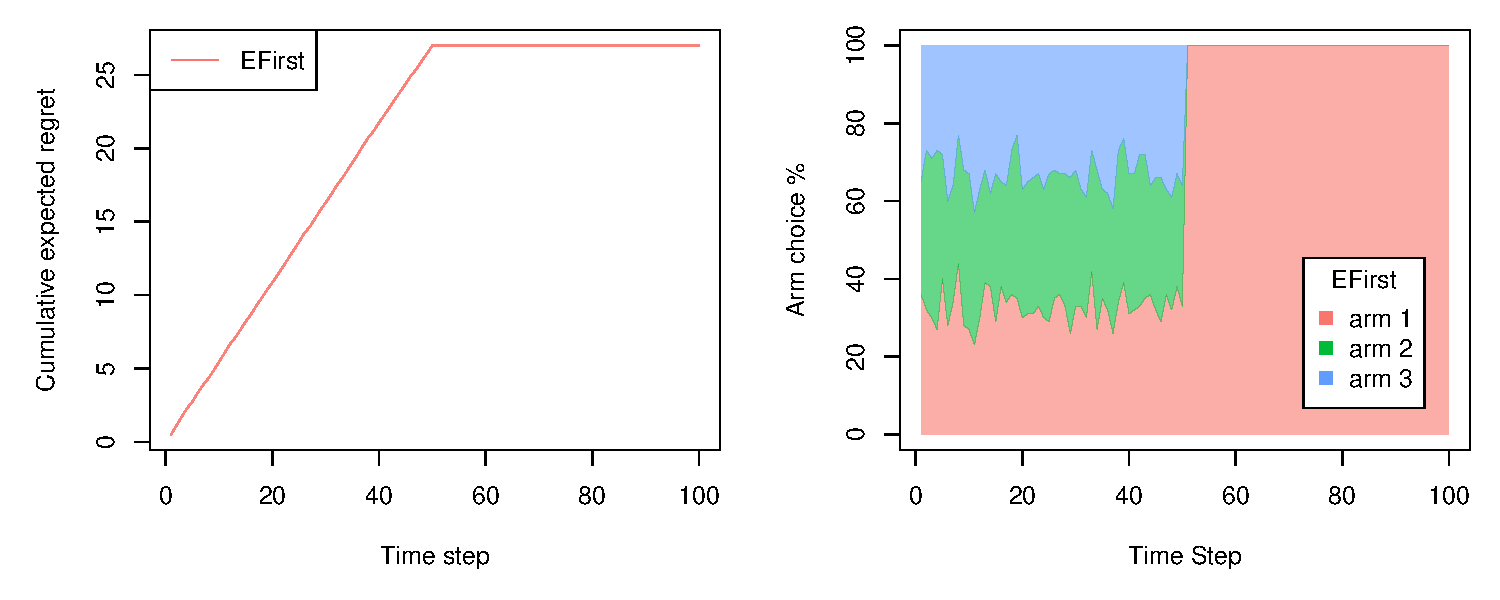
\includegraphics[width=\maxwidth,]{fig/fig1-1} \caption[Epsilon First]{Epsilon First}\label{fig:fig11}
\end{figure}

\begin{figure}[H]
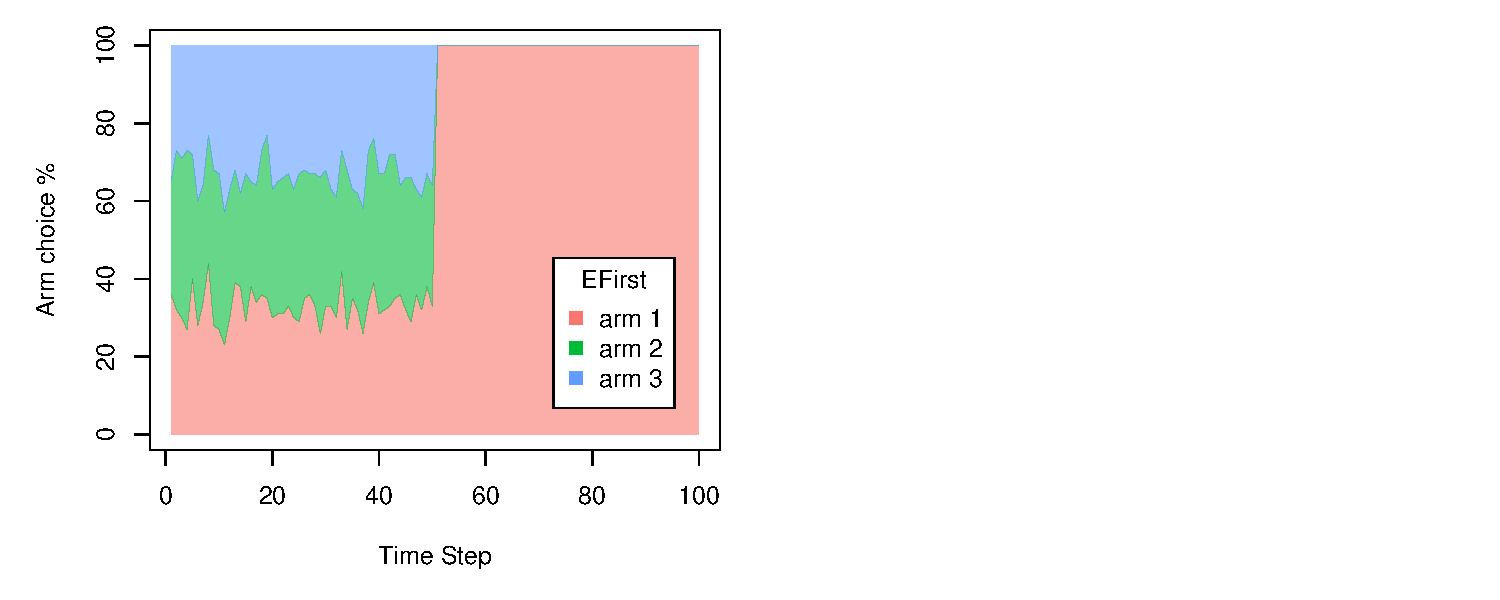
\includegraphics[width=\maxwidth,]{fig/fig1-2} \caption[Epsilon First]{Epsilon First}\label{fig:fig12}
\end{figure}


\end{knitrout}
\end{center}


\subsection{Epsilon Greedy}

This is an algorithm for continuously balancing exploration with exploitation. A randomly chosen arm is pulled a fraction $\epsilon$ of the time. The other 1-$\epsilon$ of the time, the arm with highest known payout is pulled.

For figures, see Figure \ref{fig:fig2} on page \pageref{fig:fig2}.

The algorithm:

\begin{algorithm}
\caption{Epsilon Greedy}
\label{Alg:EpsilonGreedy}
\begin{algorithmic}
\REQUIRE \(    \epsilon  \in \left[ 0,1 \right] \) - exploration tuning parameter
\STATE \( n_{a} \leftarrow 0 \) for all arms a \(  \in \left\{ 1, \dots, k \right\} \)  (count how many times an arm has been chosen)
\STATE \( \hat{\mu}_{a} \leftarrow 0 \) for all arms a  \(   \in \left\{ 1, \dots, k \right\} \)  (estimate of expected reward per arm)
% Run through time points:
\FOR{$t=1, \dots, T$}
	% Run through arms. Step 1, select which one to play
	\IF {sample from $\mathcal{N}(0,1) > \epsilon$}
		\STATE play arm \(a_t = \argmax_a  \hat{\mu}_{t-1,a}  \) with ties broken arbitrarily
	\ELSE
		\STATE play a random arm out of all arms a \(  \in \left\{ 1, \dots, k \right\} \)
	\ENDIF
	\STATE observe real-valued payoff $r_t$
	% Update:
	\STATE \( n_{a_{t}} \leftarrow n_{a_{t-1}} + 1  \)
   \STATE \( \hat{\mu}_{t,a_{t}} \leftarrow   \cfrac{r_t - \hat{\mu}_{t-1,a_{t}} }{n_{a_{t}}}   \)
\ENDFOR
\end{algorithmic}
\end{algorithm}

Translated to the EpsilonGreedyPolicy class:

\begin{knitrout}\small
\definecolor{shadecolor}{rgb}{0.969, 0.969, 0.969}\color{fgcolor}\begin{kframe}
\begin{alltt}
\hlstd{EpsilonGreedyPolicy} \hlkwb{<-} \hlstd{R6}\hlopt{::}\hlkwd{R6Class}\hlstd{(}
  \hlkwc{public} \hlstd{=} \hlkwd{list}\hlstd{(}
    \hlkwc{epsilon} \hlstd{=} \hlkwa{NULL}\hlstd{,}
    \hlkwc{initialize} \hlstd{=} \hlkwa{function}\hlstd{(}\hlkwc{epsilon} \hlstd{=} \hlnum{0.1}\hlstd{,} \hlkwc{name} \hlstd{=} \hlstr{"EGreedy"}\hlstd{) \{}
      \hlstd{super}\hlopt{$}\hlkwd{initialize}\hlstd{(name)}
      \hlstd{self}\hlopt{$}\hlstd{epsilon} \hlkwb{<-} \hlstd{epsilon}
    \hlstd{\},}
    \hlkwc{set_parameters} \hlstd{=} \hlkwa{function}\hlstd{() \{}
      \hlstd{self}\hlopt{$}\hlstd{theta_to_arms} \hlkwb{<-} \hlkwd{list}\hlstd{(}\hlstr{'n'} \hlstd{=} \hlnum{0}\hlstd{,} \hlstr{'mean'} \hlstd{=} \hlnum{0}\hlstd{)}
    \hlstd{\},}
    \hlkwc{get_action} \hlstd{=} \hlkwa{function}\hlstd{(}\hlkwc{context}\hlstd{,} \hlkwc{t}\hlstd{) \{}
      \hlkwa{if} \hlstd{(}\hlkwd{runif}\hlstd{(}\hlnum{1}\hlstd{)} \hlopt{>} \hlstd{epsilon) \{}
        \hlstd{action}\hlopt{$}\hlstd{choice} \hlkwb{<-} \hlkwd{max_in}\hlstd{(theta}\hlopt{$}\hlstd{mean)}
        \hlstd{action}\hlopt{$}\hlstd{propensity} \hlkwb{<-} \hlnum{1} \hlopt{-} \hlstd{self}\hlopt{$}\hlstd{epsilon}
      \hlstd{\}} \hlkwa{else} \hlstd{\{}
        \hlstd{action}\hlopt{$}\hlstd{choice} \hlkwb{<-} \hlkwd{sample.int}\hlstd{(context}\hlopt{$}\hlstd{k,} \hlnum{1}\hlstd{,} \hlkwc{replace} \hlstd{=} \hlnum{TRUE}\hlstd{)}
        \hlstd{action}\hlopt{$}\hlstd{propensity} \hlkwb{<-} \hlstd{epsilon}\hlopt{*}\hlstd{(}\hlnum{1}\hlopt{/}\hlstd{context}\hlopt{$}\hlstd{k)}
      \hlstd{\}}
      \hlstd{action}
    \hlstd{\},}
    \hlkwc{set_reward} \hlstd{=} \hlkwa{function}\hlstd{(}\hlkwc{context}\hlstd{,} \hlkwc{action}\hlstd{,} \hlkwc{reward}\hlstd{,} \hlkwc{t}\hlstd{) \{}
      \hlstd{arm} \hlkwb{<-} \hlstd{action}\hlopt{$}\hlstd{choice}
      \hlstd{reward} \hlkwb{<-} \hlstd{reward}\hlopt{$}\hlstd{reward}
      \hlkwd{inc}\hlstd{(theta}\hlopt{$}\hlstd{n[[arm]])}    \hlkwb{<-} \hlnum{1}
      \hlkwd{inc}\hlstd{(theta}\hlopt{$}\hlstd{mean[[arm]])} \hlkwb{<-} \hlstd{(reward} \hlopt{-} \hlstd{theta}\hlopt{$}\hlstd{mean[[arm]])} \hlopt{/} \hlstd{theta}\hlopt{$}\hlstd{n[[arm]]}
      \hlstd{theta}
    \hlstd{\}}
  \hlstd{)}
\hlstd{)}
\end{alltt}
\end{kframe}
\end{knitrout}

How to run it:

\begin{knitrout}\small
\definecolor{shadecolor}{rgb}{0.969, 0.969, 0.969}\color{fgcolor}\begin{kframe}
\begin{alltt}
\hlkwd{library}\hlstd{(}\hlstr{"contextual"}\hlstd{)}

\hlstd{horizon}            \hlkwb{<-} \hlnum{100}
\hlstd{simulations}        \hlkwb{<-} \hlnum{100}
\hlstd{weights}        \hlkwb{<-} \hlkwd{c}\hlstd{(}\hlnum{0.9}\hlstd{,} \hlnum{0.1}\hlstd{,} \hlnum{0.1}\hlstd{)}

\hlstd{policy}             \hlkwb{<-} \hlstd{EpsilonGreedyPolicy}\hlopt{$}\hlkwd{new}\hlstd{(}\hlkwc{epsilon} \hlstd{=} \hlnum{0.1}\hlstd{,} \hlkwc{name} \hlstd{=} \hlstr{"EG"}\hlstd{)}
\hlstd{bandit}             \hlkwb{<-} \hlstd{SyntheticBandit}\hlopt{$}\hlkwd{new}\hlstd{(}\hlkwc{weights} \hlstd{= weights)}

\hlstd{agent}              \hlkwb{<-} \hlstd{Agent}\hlopt{$}\hlkwd{new}\hlstd{(policy,bandit)}

\hlstd{simulator}          \hlkwb{<-} \hlstd{Simulator}\hlopt{$}\hlkwd{new}\hlstd{(}\hlkwc{agents} \hlstd{= agent,}
                                    \hlkwc{horizon} \hlstd{= horizon,}
                                    \hlkwc{simulations} \hlstd{= simulations,}
                                    \hlkwc{do_parallel} \hlstd{=} \hlnum{FALSE}\hlstd{)}

\hlstd{history}            \hlkwb{<-} \hlstd{simulator}\hlopt{$}\hlkwd{run}\hlstd{()}


\hlkwd{par}\hlstd{(}\hlkwc{mfrow} \hlstd{=} \hlkwd{c}\hlstd{(}\hlnum{1}\hlstd{,} \hlnum{2}\hlstd{),}\hlkwc{mar} \hlstd{=} \hlkwd{c}\hlstd{(}\hlnum{5}\hlstd{,} \hlnum{5}\hlstd{,} \hlnum{1}\hlstd{,} \hlnum{1}\hlstd{))}
\hlkwd{plot}\hlstd{(history,} \hlkwc{type} \hlstd{=} \hlstr{"cumulative"}\hlstd{)}
\hlkwd{plot}\hlstd{(history,} \hlkwc{type} \hlstd{=} \hlstr{"arms"}\hlstd{)}
\end{alltt}
\end{kframe}
\end{knitrout}

\begin{center}
\begin{knitrout}
\definecolor{shadecolor}{rgb}{0.969, 0.969, 0.969}\color{fgcolor}\begin{figure}[H]
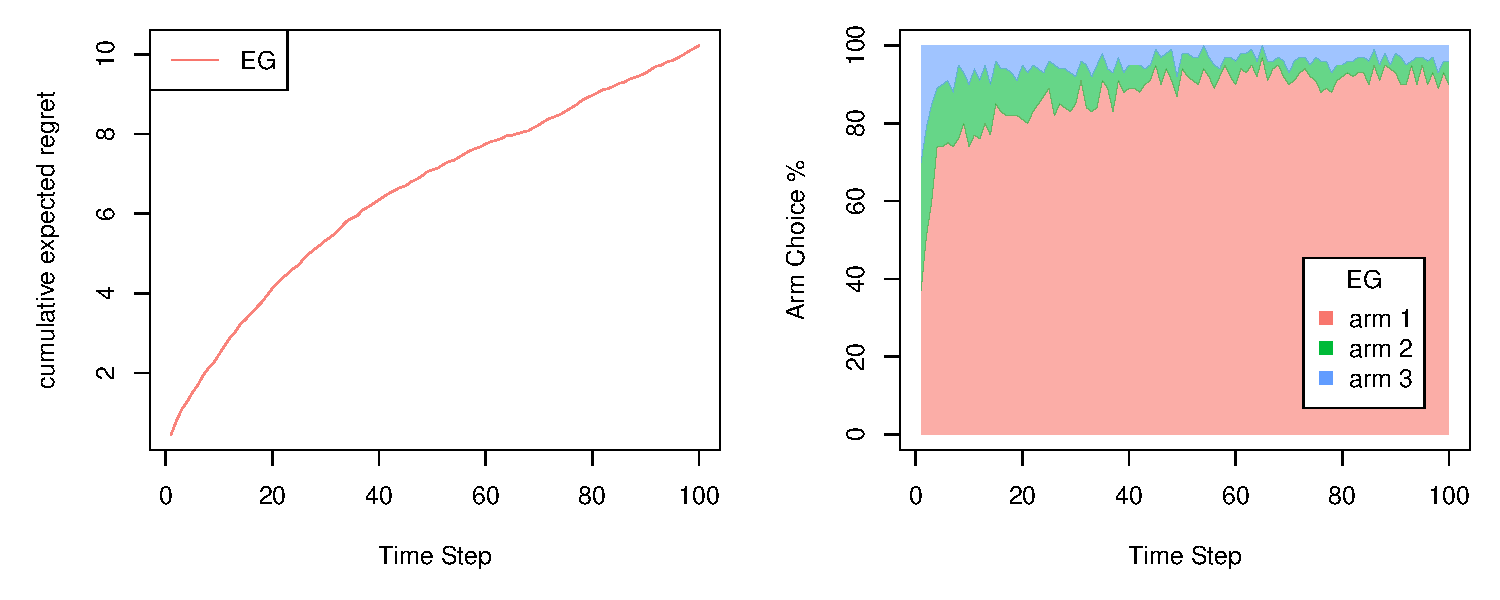
\includegraphics[width=\maxwidth,]{fig/fig2-1} \caption[Epsilon Greedy]{Epsilon Greedy}\label{fig:fig21}
\end{figure}

\begin{figure}[H]
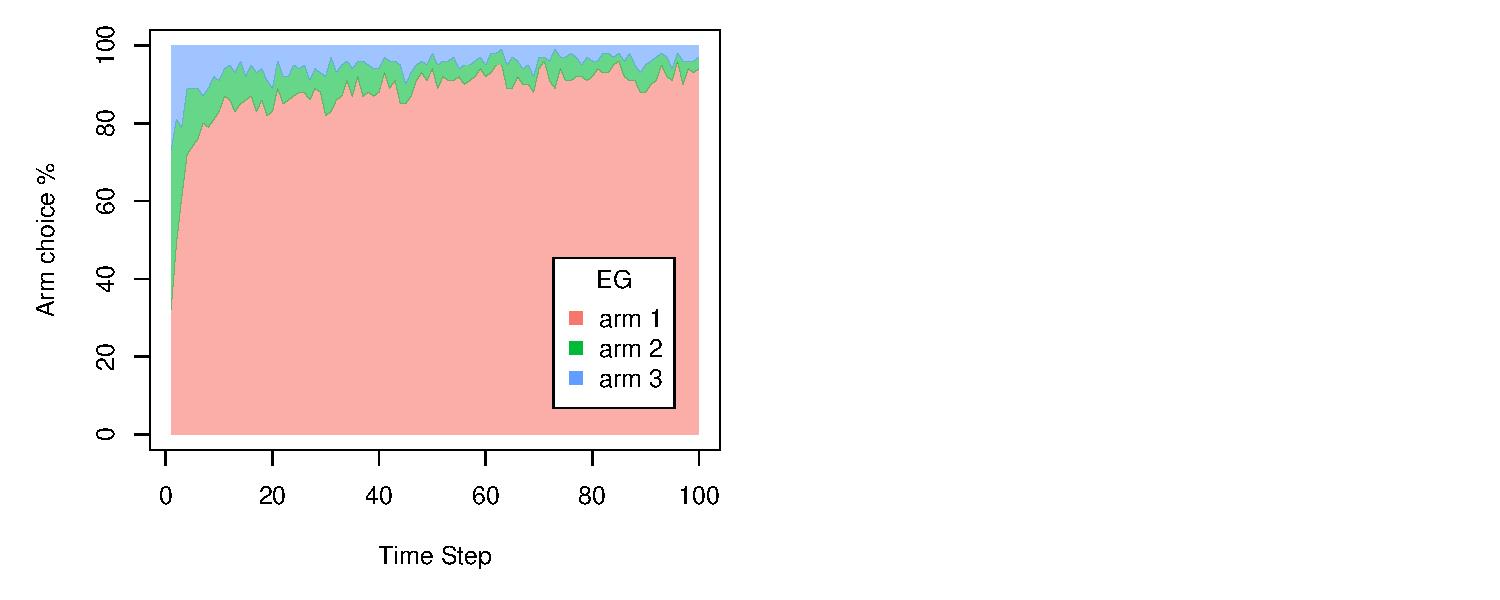
\includegraphics[width=\maxwidth,]{fig/fig2-2} \caption[Epsilon Greedy]{Epsilon Greedy}\label{fig:fig22}
\end{figure}


\end{knitrout}
\end{center}

\subsection{Contextual Bandit: LinUCB with Linear Disjoint Models}

The algorithm:

\begin{algorithm}
\caption{LinUCB with linear disjoint models}
\label{Alg:LinUCBDisjoint}
\begin{algorithmic}
\REQUIRE $\alpha$ \(  \in \mathbb{R}^{+} \), exploration tuning parameter
% Run through time points:
\FOR{$t=1, \dots, T$}
          \STATE Observe features of all arms \(  a \in \mathcal{A}_{t}: x_{t,a} \in \mathbb{R}^{d}\)
	% Run through arms. Step 1, select which one to play
	\FOR{ \(  a \in \mathcal{A}_{t}\)}
	          \IF{\(a\) is new}
		      \STATE \(A_{a} \leftarrow I_{d}  \)  (d-dimensional identity matrix)
		      \STATE \(b_{a} \leftarrow 0_{d\times1}   \) (d-dimensional zero vector)
		\ENDIF
		\STATE \( \hat{\theta}_{a} \leftarrow A_{a}^{-1}b_{a} \)
		\STATE \( p_{t,a} \leftarrow \hat{\theta}_{a}^{T} + \alpha  \sqrt{ x_{t,a}^{T} A_{a}^{-1}x_{t,a}} \)
	\ENDFOR
	% allocate to arm
	\STATE Play arm \(a_t = \argmax_a  p_{t,a}  \) with ties broken arbitrarily and observe real-valued payoff $r_t$
	% Update:
           \STATE \( A_{a_{t}} \leftarrow A_{a_{t}}+ x_{t,a_{t}}x_{t,a_{t}}^{T} \)
           \STATE  \( b_{a_{t}} \leftarrow b_{a_{t}}+ r_{t}x_{t,a_{t}}  \)
\ENDFOR
\end{algorithmic}
\end{algorithm}

This is how the algorithm works: at each step, we run a linear regression with the data we have collected so far such that we have a coefficient for each context feature. We then observe our new context, and generate a predicted payoff using our model. We also generate a confidence interval for that predicted payoff for each of the three arms. We then choose the arm with the highest upper confidence bound.

For figures, see Figure \ref{fig:fig3} on page \pageref{fig:fig3}.

\begin{knitrout}\small
\definecolor{shadecolor}{rgb}{0.969, 0.969, 0.969}\color{fgcolor}\begin{kframe}
\begin{alltt}
\hlcom{#' @export}
\hlstd{LinUCBDisjointPolicy} \hlkwb{<-} \hlstd{R6}\hlopt{::}\hlkwd{R6Class}\hlstd{(}
  \hlkwc{public} \hlstd{=} \hlkwd{list}\hlstd{(}
    \hlkwc{alpha} \hlstd{=} \hlkwa{NULL}\hlstd{,}
    \hlkwc{initialize} \hlstd{=} \hlkwa{function}\hlstd{(}\hlkwc{alpha} \hlstd{=} \hlnum{1.0}\hlstd{,} \hlkwc{name} \hlstd{=} \hlstr{"LinUCBDisjoint"}\hlstd{) \{}
      \hlstd{super}\hlopt{$}\hlkwd{initialize}\hlstd{(name)}
      \hlstd{self}\hlopt{$}\hlstd{alpha} \hlkwb{<-} \hlstd{alpha}
    \hlstd{\},}
    \hlkwc{set_parameters} \hlstd{=} \hlkwa{function}\hlstd{() \{}
      \hlstd{self}\hlopt{$}\hlstd{theta_to_arms} \hlkwb{<-} \hlkwd{list}\hlstd{(} \hlstr{'A'} \hlstd{=} \hlkwd{diag}\hlstd{(}\hlnum{1}\hlstd{,self}\hlopt{$}\hlstd{d,self}\hlopt{$}\hlstd{d),} \hlstr{'b'} \hlstd{=} \hlkwd{rep}\hlstd{(}\hlnum{0}\hlstd{,self}\hlopt{$}\hlstd{d))}
    \hlstd{\},}
    \hlkwc{get_action} \hlstd{=} \hlkwa{function}\hlstd{(}\hlkwc{context}\hlstd{,} \hlkwc{t}\hlstd{) \{}
      \hlstd{expected_rewards} \hlkwb{<-} \hlkwd{rep}\hlstd{(}\hlnum{0.0}\hlstd{, context}\hlopt{$}\hlstd{k)}
      \hlkwa{for} \hlstd{(arm} \hlkwa{in} \hlnum{1}\hlopt{:}\hlstd{self}\hlopt{$}\hlstd{k) \{}
        \hlstd{X}          \hlkwb{<-}  \hlstd{context}\hlopt{$}\hlstd{X[,arm]}
        \hlstd{A}          \hlkwb{<-}  \hlstd{theta}\hlopt{$}\hlstd{A[[arm]]}
        \hlstd{b}          \hlkwb{<-}  \hlstd{theta}\hlopt{$}\hlstd{b[[arm]]}
        \hlstd{A_inv}      \hlkwb{<-}  \hlkwd{solve}\hlstd{(A)}

        \hlstd{theta_hat}  \hlkwb{<-}  \hlstd{A_inv} \hlopt \hlstd{b}
        \hlstd{mean}       \hlkwb{<-}  \hlstd{X} \hlopt \hlstd{theta_hat}
        \hlstd{sd}         \hlkwb{<-}  \hlkwd{sqrt}\hlstd{(}\hlkwd{tcrossprod}\hlstd{(X} \hlopt \hlstd{A_inv, X))}
        \hlstd{expected_rewards[arm]} \hlkwb{<-} \hlstd{mean} \hlopt{+} \hlstd{alpha} \hlopt{*} \hlstd{sd}
      \hlstd{\}}
      \hlstd{action}\hlopt{$}\hlstd{choice}  \hlkwb{<-} \hlkwd{max_in}\hlstd{(expected_rewards)}
      \hlstd{action}
    \hlstd{\},}
    \hlkwc{set_reward} \hlstd{=} \hlkwa{function}\hlstd{(}\hlkwc{context}\hlstd{,} \hlkwc{action}\hlstd{,} \hlkwc{reward}\hlstd{,} \hlkwc{t}\hlstd{) \{}
      \hlstd{arm} \hlkwb{<-} \hlstd{action}\hlopt{$}\hlstd{choice}
      \hlstd{reward} \hlkwb{<-} \hlstd{reward}\hlopt{$}\hlstd{reward}
      \hlstd{Xa} \hlkwb{<-} \hlstd{context}\hlopt{$}\hlstd{X[,arm]}

      \hlkwd{inc}\hlstd{(theta}\hlopt{$}\hlstd{A[[arm]])} \hlkwb{<-} \hlkwd{outer}\hlstd{(Xa, Xa)}
      \hlkwd{inc}\hlstd{(theta}\hlopt{$}\hlstd{b[[arm]])} \hlkwb{<-} \hlstd{reward} \hlopt{*} \hlstd{Xa}

      \hlstd{theta}
    \hlstd{\}}
  \hlstd{)}
\hlstd{)}
\end{alltt}
\end{kframe}
\end{knitrout}


\begin{knitrout}\small
\definecolor{shadecolor}{rgb}{0.969, 0.969, 0.969}\color{fgcolor}\begin{kframe}
\begin{alltt}
\hlstd{horizon}          \hlkwb{<-} \hlnum{100L}
\hlstd{simulations}      \hlkwb{<-} \hlnum{300L}
                              \hlcom{# k=1  k=2  k=3           columns represent arms}
\hlstd{weights}  \hlkwb{<-} \hlkwd{matrix}\hlstd{(}          \hlkwd{c}\hlstd{(} \hlnum{0.9}\hlstd{,} \hlnum{0.1}\hlstd{,} \hlnum{0.1}\hlstd{,}  \hlcom{# d=1}
                                \hlnum{0.1}\hlstd{,} \hlnum{0.9}\hlstd{,} \hlnum{0.1}\hlstd{,}  \hlcom{# d=2}
                                \hlnum{0.1}\hlstd{,} \hlnum{0.1}\hlstd{,} \hlnum{0.9}\hlstd{),} \hlcom{# d=3   rows for context features}

                                \hlkwc{nrow} \hlstd{=} \hlnum{3}\hlstd{,} \hlkwc{ncol} \hlstd{=} \hlnum{3}\hlstd{,} \hlkwc{byrow} \hlstd{=} \hlnum{TRUE}\hlstd{)}

\hlstd{bandit}             \hlkwb{<-} \hlstd{SyntheticBandit}\hlopt{$}\hlkwd{new}\hlstd{(}\hlkwc{weights} \hlstd{= weights,} \hlkwc{precaching} \hlstd{=} \hlnum{TRUE}\hlstd{)}

\hlstd{agents}             \hlkwb{<-} \hlkwd{list}\hlstd{( Agent}\hlopt{$}\hlkwd{new}\hlstd{(EpsilonGreedyPolicy}\hlopt{$}\hlkwd{new}\hlstd{(}\hlnum{0.1}\hlstd{,} \hlstr{"EpsilonGreedy"}\hlstd{), bandit),}
                            \hlstd{Agent}\hlopt{$}\hlkwd{new}\hlstd{(LinUCBDisjointPolicy}\hlopt{$}\hlkwd{new}\hlstd{(}\hlnum{1.0}\hlstd{,} \hlstr{"LinUCB"}\hlstd{), bandit) )}

\hlstd{simulation}         \hlkwb{<-} \hlstd{Simulator}\hlopt{$}\hlkwd{new}\hlstd{(agents, horizon, simulations,} \hlkwc{do_parallel} \hlstd{=} \hlnum{FALSE}\hlstd{)}
\hlstd{history}            \hlkwb{<-} \hlstd{simulation}\hlopt{$}\hlkwd{run}\hlstd{()}

\hlkwd{par}\hlstd{(}\hlkwc{mfrow} \hlstd{=} \hlkwd{c}\hlstd{(}\hlnum{1}\hlstd{,} \hlnum{2}\hlstd{),}\hlkwc{mar} \hlstd{=} \hlkwd{c}\hlstd{(}\hlnum{5}\hlstd{,} \hlnum{5}\hlstd{,} \hlnum{1}\hlstd{,} \hlnum{1}\hlstd{))}
\hlkwd{plot}\hlstd{(history,} \hlkwc{type} \hlstd{=} \hlstr{"cumulative"}\hlstd{)}
\hlkwd{plot}\hlstd{(history,} \hlkwc{type} \hlstd{=} \hlstr{"cumulative"}\hlstd{,} \hlkwc{regret} \hlstd{=} \hlnum{FALSE}\hlstd{)}
\end{alltt}
\end{kframe}
\end{knitrout}

\begin{center}
\begin{knitrout}
\definecolor{shadecolor}{rgb}{0.969, 0.969, 0.969}\color{fgcolor}\begin{figure}[H]
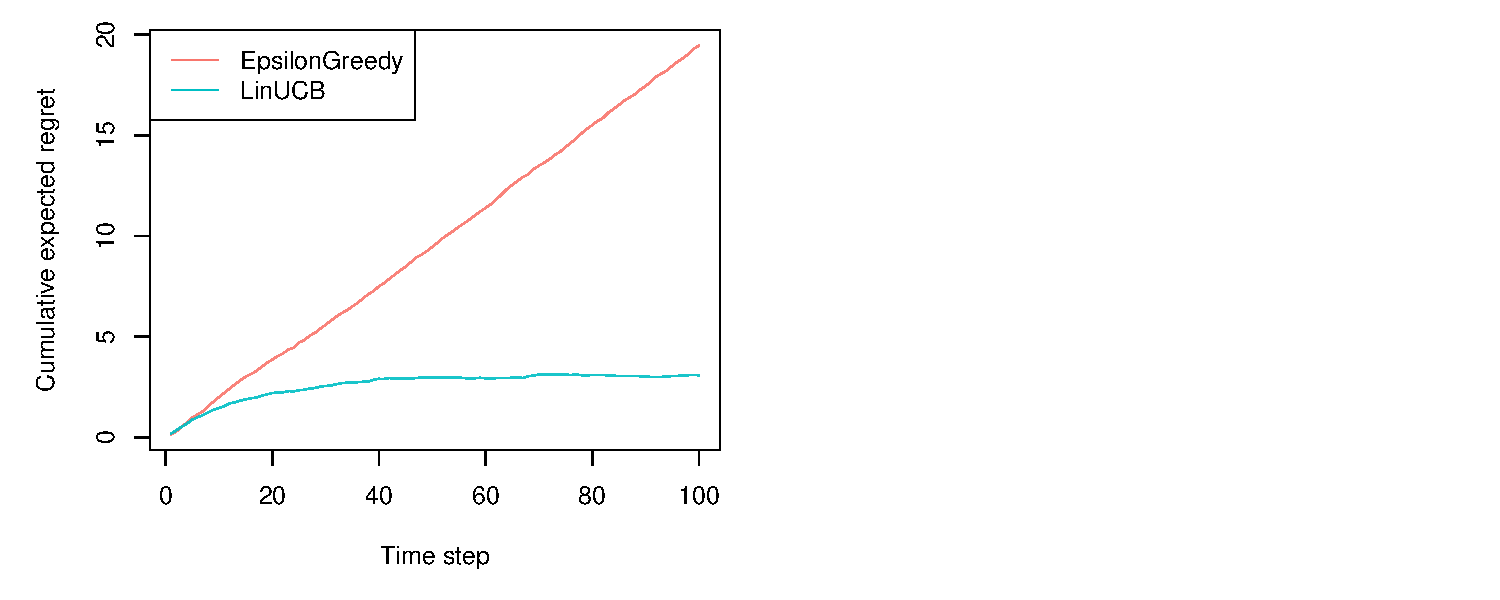
\includegraphics[width=\maxwidth,]{fig/fig3-1} \caption[LinUCB algorithm with linear disjoint models, following Li et al]{LinUCB algorithm with linear disjoint models, following Li et al. (2010)}\label{fig:fig31}
\end{figure}

\begin{figure}[H]
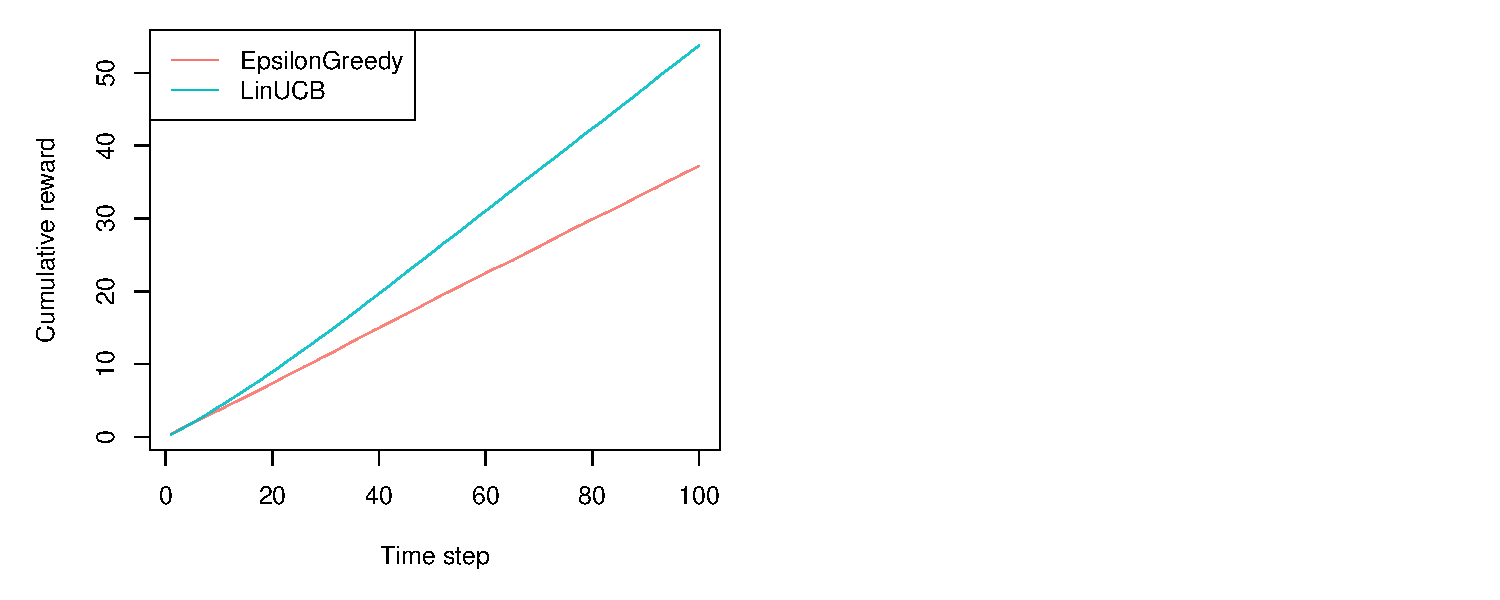
\includegraphics[width=\maxwidth,]{fig/fig3-2} \caption[LinUCB algorithm with linear disjoint models, following Li et al]{LinUCB algorithm with linear disjoint models, following Li et al. (2010)}\label{fig:fig32}
\end{figure}


\end{knitrout}
\end{center}

\section{Extending the package}

Through its R6 based object system, it's relatively easy to extend \pkg{contextual}. Below, we demonstrate how to make use of that extensibility through the implementation of a PoissonRewardBandit extending \pkg{contextual}'s BasicBandit class, and of an PoissonRewardBandit version of the Epsilon Greedy policy presented above.

\begin{knitrout}\small
\definecolor{shadecolor}{rgb}{0.969, 0.969, 0.969}\color{fgcolor}\begin{kframe}
\begin{alltt}
\hlstd{PoissonRewardBandit} \hlkwb{<-} \hlstd{R6}\hlopt{::}\hlkwd{R6Class}\hlstd{(}
  \hlstr{"PoissonRewardBandit"}\hlstd{,}
  \hlcom{# Class extends BasicBandit}
  \hlkwc{inherit} \hlstd{= BasicBandit,}
  \hlkwc{public} \hlstd{=} \hlkwd{list}\hlstd{(}
    \hlkwc{initialize} \hlstd{=} \hlkwa{function}\hlstd{(}\hlkwc{weights}\hlstd{) \{}
      \hlstd{super}\hlopt{$}\hlkwd{initialize}\hlstd{(weights)}
    \hlstd{\},}
    \hlcom{# Overrides BasicBandit's do_action to generate Poisson based rewards}
    \hlkwc{do_action} \hlstd{=} \hlkwa{function}\hlstd{(}\hlkwc{context}\hlstd{,} \hlkwc{action}\hlstd{,} \hlkwc{t}\hlstd{) \{}
      \hlstd{reward_means} \hlkwb{=} \hlkwd{c}\hlstd{(}\hlnum{2}\hlstd{,}\hlnum{2}\hlstd{,}\hlnum{2}\hlstd{)}
      \hlstd{private}\hlopt{$}\hlstd{R} \hlkwb{<-} \hlkwd{matrix}\hlstd{(}\hlkwd{rpois}\hlstd{(}\hlnum{3}\hlstd{, reward_means)} \hlopt{<} \hlstd{self}\hlopt{$}\hlkwd{get_weights}\hlstd{(), self}\hlopt{$}\hlstd{k, self}\hlopt{$}\hlstd{d)}\hlopt{*}\hlnum{1}
      \hlkwd{list}\hlstd{(}
        \hlkwc{reward}                   \hlstd{= private}\hlopt{$}\hlstd{R[action}\hlopt{$}\hlstd{choice],}
        \hlkwc{optimal_reward_value}     \hlstd{= private}\hlopt{$}\hlstd{R[}\hlkwd{which.max}\hlstd{(private}\hlopt{$}\hlstd{R)]}
      \hlstd{)}
    \hlstd{\}}
  \hlstd{)}
\hlstd{)}
\hlstd{EpsilonGreedyAnnealingPolicy} \hlkwb{<-} \hlstd{R6}\hlopt{::}\hlkwd{R6Class}\hlstd{(}
  \hlstr{"EpsilonGreedyAnnealingPolicy"}\hlstd{,}
  \hlcom{# Class extends EpsilonGreedyPolicy}
  \hlkwc{inherit} \hlstd{= EpsilonGreedyPolicy,}
  \hlkwc{portable} \hlstd{=} \hlnum{TRUE}\hlstd{,}
  \hlkwc{class} \hlstd{=} \hlnum{TRUE}\hlstd{,}
  \hlkwc{public} \hlstd{=} \hlkwd{list}\hlstd{(}
    \hlcom{# Override get_action, use annealing epsilon}
    \hlkwc{get_action} \hlstd{=} \hlkwa{function}\hlstd{(}\hlkwc{context}\hlstd{,} \hlkwc{t}\hlstd{) \{}
      \hlstd{self}\hlopt{$}\hlstd{epsilon} \hlkwb{<-} \hlnum{1} \hlopt{/} \hlkwd{log}\hlstd{(t} \hlopt{+} \hlnum{0.0000001}\hlstd{)}
      \hlstd{super}\hlopt{$}\hlkwd{get_action}\hlstd{(context, t)}
    \hlstd{\}}
  \hlstd{)}
\hlstd{)}

\hlstd{weights}     \hlkwb{<-} \hlkwd{c}\hlstd{(}\hlnum{7}\hlstd{,}\hlnum{1}\hlstd{,}\hlnum{2}\hlstd{)}
\hlstd{bandit}      \hlkwb{<-} \hlstd{PoissonRewardBandit}\hlopt{$}\hlkwd{new}\hlstd{(weights)}
\hlstd{agents}      \hlkwb{<-} \hlkwd{list}\hlstd{( Agent}\hlopt{$}\hlkwd{new}\hlstd{(EpsilonGreedyPolicy}\hlopt{$}\hlkwd{new}\hlstd{(}\hlnum{0.1}\hlstd{,} \hlstr{"EG Annealing"}\hlstd{), bandit),}
                     \hlstd{Agent}\hlopt{$}\hlkwd{new}\hlstd{(EpsilonGreedyAnnealingPolicy}\hlopt{$}\hlkwd{new}\hlstd{(}\hlnum{0.1}\hlstd{,} \hlstr{"EG"}\hlstd{), bandit) )}
\end{alltt}


{\ttfamily\noindent\bfseries\color{errorcolor}{\#\# Error in EpsilonGreedyAnnealingPolicy\$new(0.1, "{}EG"{}): Sub and superclass must both be portable or non-portable.}}\begin{alltt}
\hlstd{simulation}  \hlkwb{<-} \hlstd{Simulator}\hlopt{$}\hlkwd{new}\hlstd{(agents,} \hlkwc{horizon} \hlstd{=} \hlnum{200L}\hlstd{,} \hlkwc{simulations} \hlstd{=} \hlnum{100L}\hlstd{,} \hlkwc{do_parallel} \hlstd{=} \hlnum{FALSE}\hlstd{)}

\hlstd{history}     \hlkwb{<-} \hlstd{simulation}\hlopt{$}\hlkwd{run}\hlstd{()}

\hlkwd{par}\hlstd{(}\hlkwc{mfrow} \hlstd{=} \hlkwd{c}\hlstd{(}\hlnum{1}\hlstd{,} \hlnum{2}\hlstd{),}\hlkwc{mar} \hlstd{=} \hlkwd{c}\hlstd{(}\hlnum{5}\hlstd{,} \hlnum{5}\hlstd{,} \hlnum{1}\hlstd{,} \hlnum{1}\hlstd{))}
\hlkwd{plot}\hlstd{(history,} \hlkwc{type} \hlstd{=} \hlstr{"cumulative"}\hlstd{)}
\hlkwd{plot}\hlstd{(history,} \hlkwc{type} \hlstd{=} \hlstr{"average"}\hlstd{,} \hlkwc{regret} \hlstd{=} \hlnum{FALSE}\hlstd{)}
\end{alltt}
\end{kframe}
\end{knitrout}

\begin{center}
\begin{knitrout}
\definecolor{shadecolor}{rgb}{0.969, 0.969, 0.969}\color{fgcolor}\begin{kframe}


{\ttfamily\noindent\bfseries\color{errorcolor}{\#\# Error in EpsilonGreedyAnnealingPolicy\$new(0.1, "{}EG"{}): Sub and superclass must both be portable or non-portable.}}\end{kframe}\begin{figure}[H]
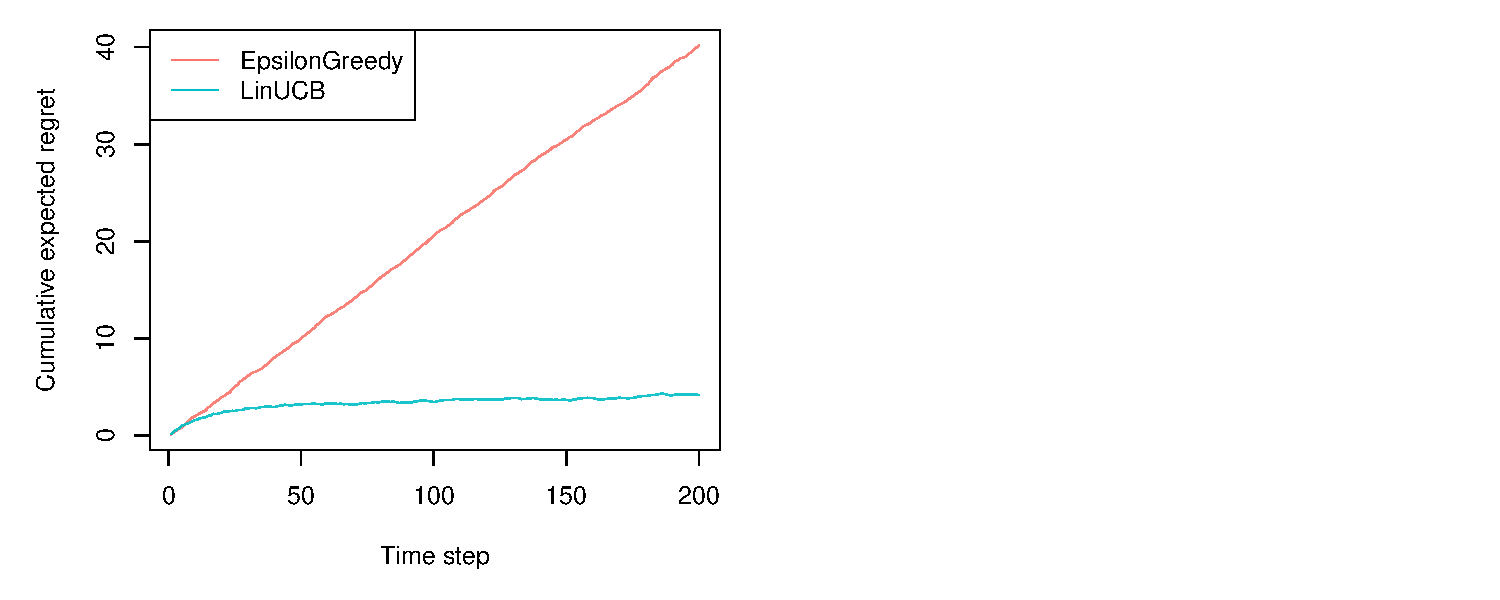
\includegraphics[width=\maxwidth,]{fig/fig4-1} \caption[Extending BasicBandit and EpsilonGreedyPolicy]{Extending BasicBandit and EpsilonGreedyPolicy}\label{fig:fig41}
\end{figure}

\begin{figure}[H]
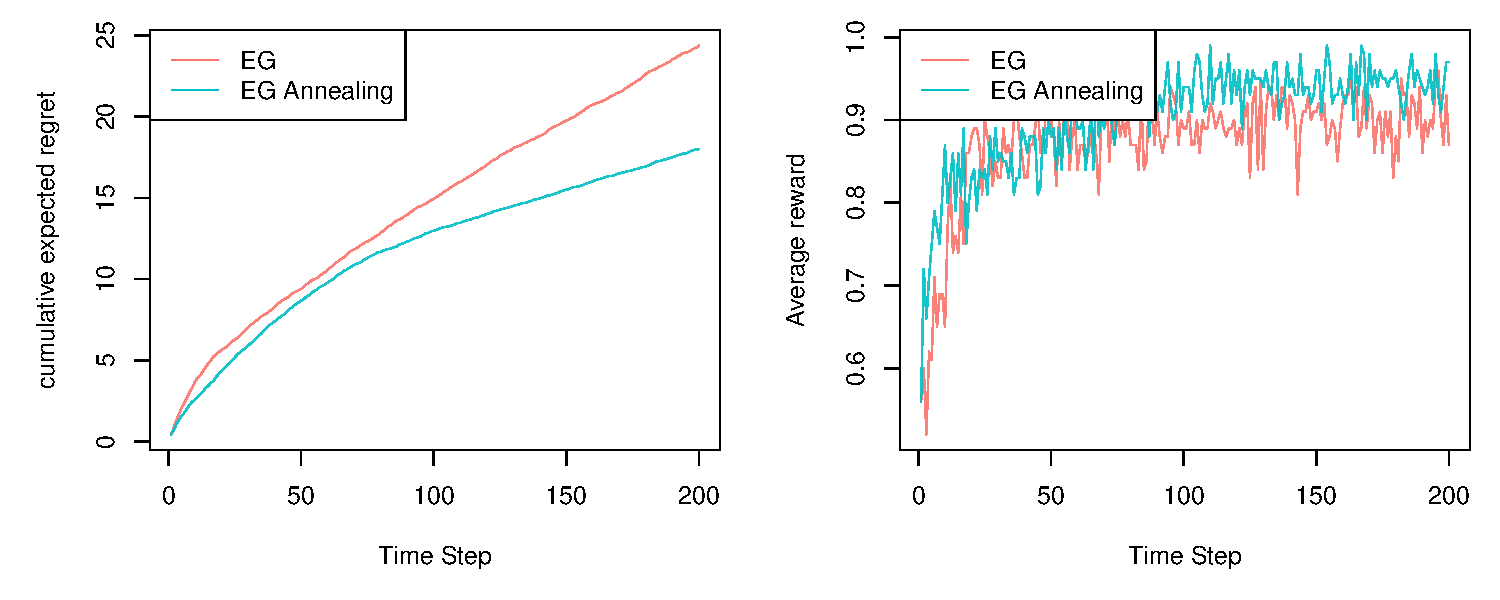
\includegraphics[width=\maxwidth,]{fig/fig4-2} \caption[Extending BasicBandit and EpsilonGreedyPolicy]{Extending BasicBandit and EpsilonGreedyPolicy}\label{fig:fig42}
\end{figure}


\end{knitrout}
\end{center}


\section{Simulation and Offline evaluation Bandits}

\subsection{Simulation}

Some info on the implemented simulating Bandits, inc strengths and weakenesses.

*** Basic very simple ***

*** Based on modeling ***

\subsection{Offline evaluation}

\subsubsection{Offline evaluation through LiLogBandit}

Though it is, as demonstrated in the previous section, relatively easy to create basic simulators to test simple MAB and cMAB policies, the creation of more complex simulations that generate more complex contexts for more demanding policies can become very complicated very fast. So much so, that the implementation of such simulators regularly becomes more complex than the analysis and implementation of the policies themselves. More seriously, even when succeeding in surpassing these technical challenges, it remains an open question if an evaluation based on simulated data reflects real-world applications, as modeling by definition introduces bias.

But there exists another, unbiased approach to testing MAB and cMAB policies. This approach makes use of widely available offline sources of data and can pre-empt the issues of bias and model complexity. It also offers the secondary advantages that offline data is both widely available and reflective of real-world online interactions. But there is one catch, that is particular to the evaluation of MAB problems: when we seek to make use of offline data, we miss out on user feedback when a policy advices a different arm than the one the user selected. In other words, offline data is only "partially labeled" with respect to any Bandit policies, as bandit evaluations only contain user feedback for arms that were displayed to the agent but include no information on other arms.

*** explain how li log algorithm helps here***

*** insert algorithm ***


*** insert code ***


\subsubsection{Offline evaluation through DoublyRobustBandit}



*** insert algorithm ***


*** insert code ***

\section{Replications with offline data}

Here we replicate some papers with a huge offline dataset..

\begin{figure}[H]
  \centering
    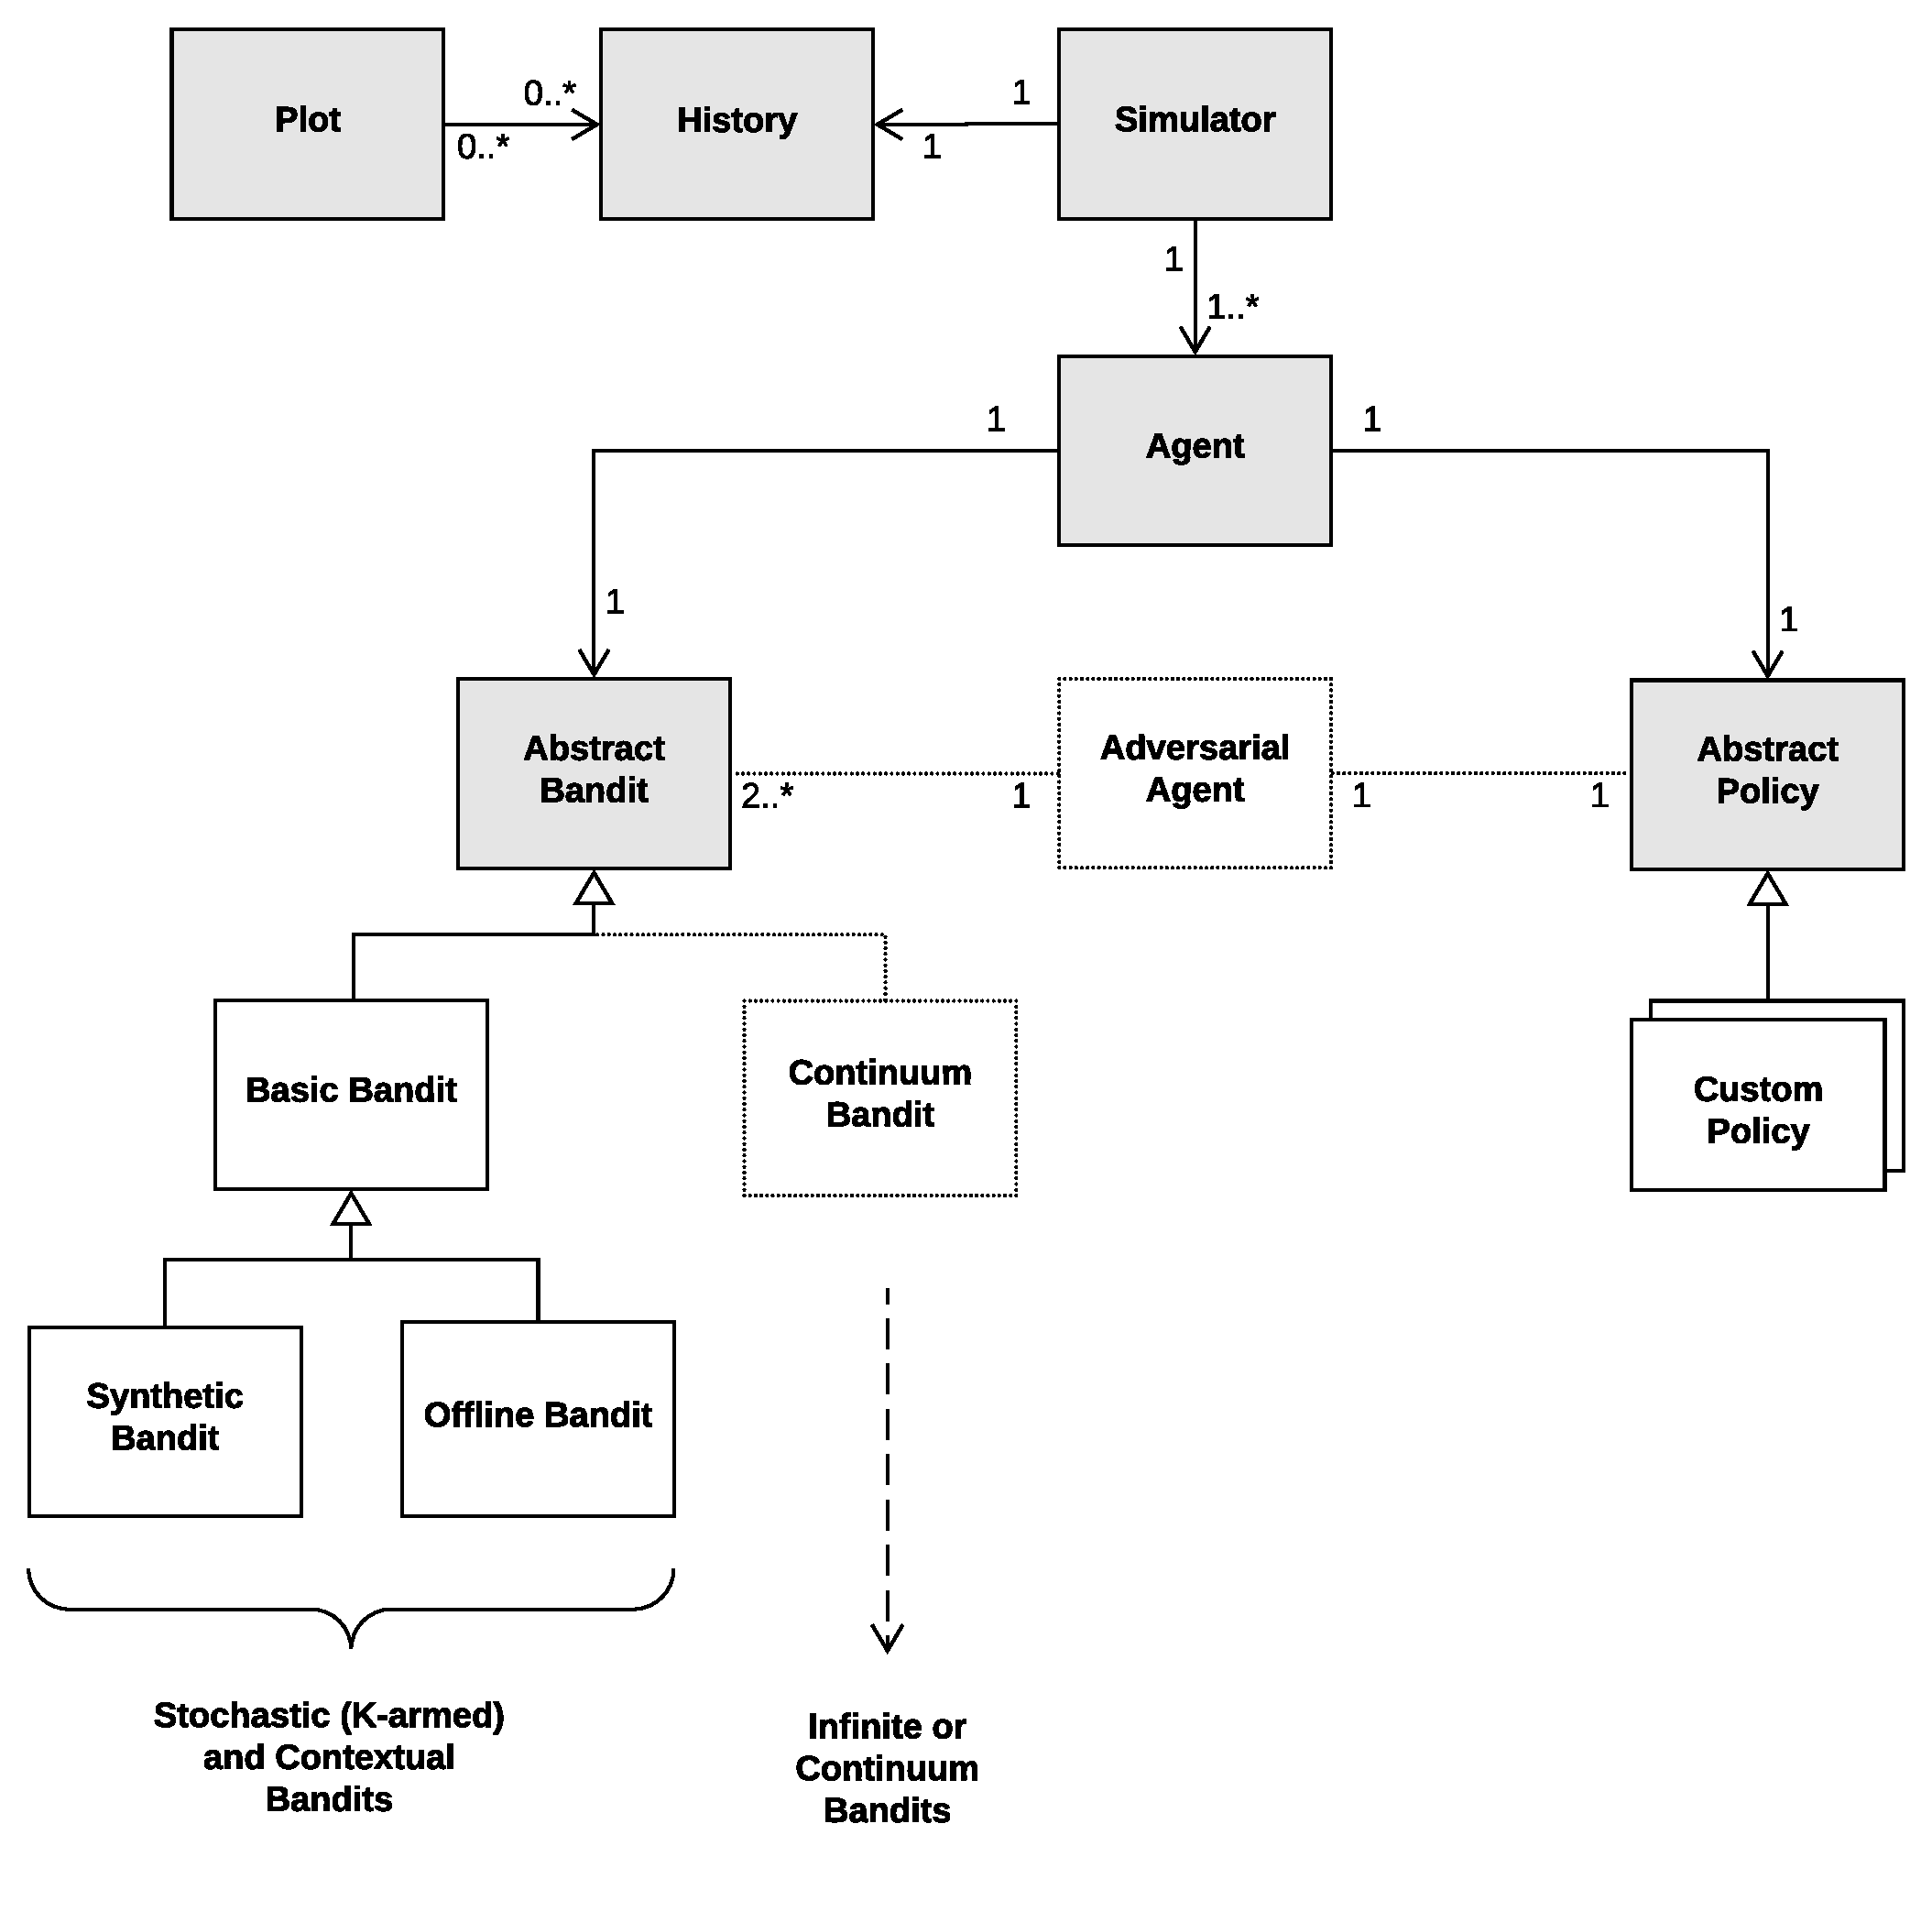
\includegraphics[width=.99\textwidth]{fig/contextual_class}
    \label{fig:contextual_class}
      \caption{\pkg{contextual} UML Class Diagram}
\end{figure}

\begin{figure}[H]
  \centering
    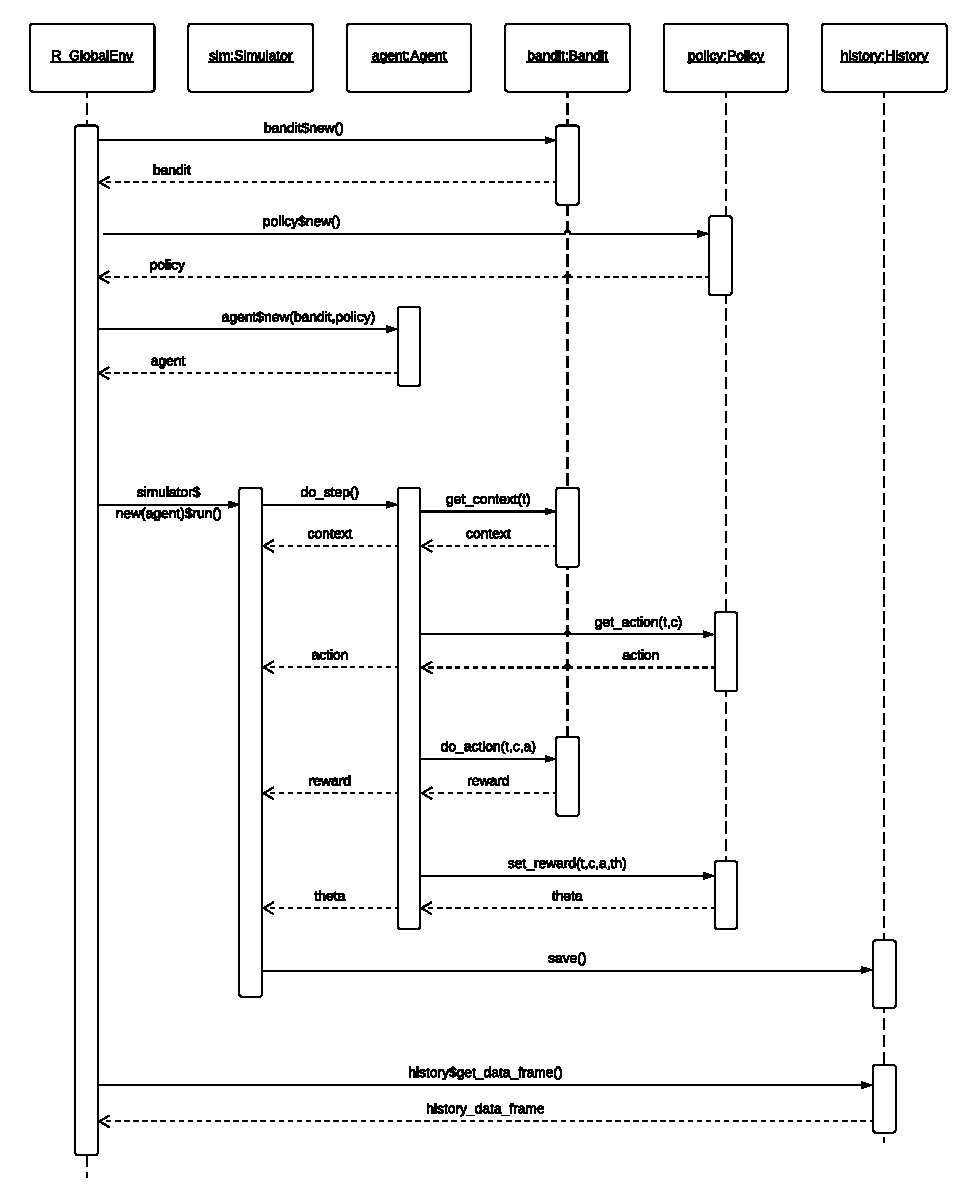
\includegraphics[width=.99\textwidth]{fig/contextual_sequence}
    \label{fig:contextual_sequence}
      \caption{\pkg{contextual} UML Sequence Diagram}
\end{figure}

\section{Special features}
%% Note: If there is markup in \(sub)section, then it has to be escape as above.

For instance, quantifying variance..

\section{The art of optimal parallelisation}
%% Note: If there is markup in \(sub)section, then it has to be escape as above.

There is a very intersting trade of between the amount of parallelisation (how many cores, nodes used) the resources needed to compute a certain model, and the amount of data going to and fro the cores.

PERFORMANCE DATA  ------------------------------------------------------------

on 58  cores:    k3*d3 * 5 policies * 300  * 10000 --\textgreater{} 132 seconds

on 120 cores:    k3*d3 * 5 policies * 300  * 10000 --\textgreater{} 390 seconds

---

on 58  cores:    k3*d3 * 5 policies * 3000 * 10000 --\textgreater{} 930 seconds

on 120 cores:    k3*d3 * 5 policies * 3000 * 10000 --\textgreater{} 691 seconds



\section{Extra greedy UCB}
%% Note: If there is markup in \(sub)section, then it has to be escape as above.

Ladila bladibla.

\section{Conclusions}
\label{sec:conc4}


Placeholder... the goal of a data analysis is not only to answer a research question based on data but also to collect findings that support that answer. These findings usually take the form of a~table, plot or regression/classification model and are usually presented in articles or reports.

\section{Acknowledgments}

Thanks go to CCC.

%\bibliographystyle{apacite}
\bibliography{jss}

\end{document}
